\documentclass[linenumbers,RNAAS,trackchanges]{aastex631}
\usepackage[utf8]{inputenc}
\usepackage{hyperref}           % hrefs
\usepackage{natbib}             % for bibliography
\usepackage{float}              % figure positioning
\usepackage{svg}                % used for SVG images
\usepackage{graphicx}           % used for non-SVG images
\usepackage{csvsimple}
% Search Query Metadata
\shorttitle{N-Body Simulations of Galaxy Interactions}
\shortauthors{Ajaykumar, et al.}

% Hyperlink setup
\hypersetup{
colorlinks=true,
linkcolor=blue,
urlcolor=blue
}

\begin{document}
\title{Using N-Body Simulations to Investigate Galaxy Interactions}
% [] is for ORCiD
\correspondingauthor{}
\email{nikhitaajaykumar@utexas.edu, khernandez@utexas.edu, darryl.tran@utexas.edu}
\author{Nikhita Ajaykumar}

\author{Kayla Hernandez}

% or 
% \nocollaboration{0}

\author{Darryl Tran}
\affiliation{University of Texas at Austin\\
110 Inner Campus Drive\\
Austin, TX 78705}

% 250 word limit for abstract
\begin{abstract}
Galaxy interactions explain morphology, color, star formation, and other composing factors within galaxies. Various computational methods have been used to create N-body simulations of galaxy interactions. These investigations have led to many discoveries of galaxy and star formation. This paper will be running various investigations using N-body simulations to better understand galaxy interactions and view how accurately the simulations match observable phenomena. 
\end{abstract}

% Use astrothesaurus numbers in place of num
\keywords{N-body Simulation (1) --- Galaxy Interactions (2) --- Computational Astrophysics (3)}
\section{Introduction} \label{sec:intro}
Interacting galaxies are galaxies whose gravitational fields interact with each other, leading to disturbances like collisions. Galaxy interactions contribute to the morphology, color, star formation, gas content, and overall composition of the galaxy\cite{das}. Galaxy collisions have been implicated in star formation and have been theorized to trigger supermassive black holes \cite{das} \cite{goulding}. Large galaxies have been thought to result from collisions between smaller galaxies. N-body simulations of galaxy interactions can be used to study the formation of such phenomena.

Pioneering simulations were done through the work of Erik Holmberg (1941) preceding the introduction of supercomputers.\cite{nbod} His innovative design included the use of lightbulbs to mimic star clusters and he found a direction by which he could calculate the forces between the stars.\cite{nbod} Later on, Alar and Jurij Toomre (1972) conducted the first computer simulations of galaxy interactions.\cite{nbod} Although the computers were not equipped to handle large sizes of particles, their simulations were able to recreate how many galaxies were formed and also led to the understanding of how tidal tails are formed.\cite{nbod} Simulations of galaxy interactions have continued to develop and are now used in the field of computational astrophysics. One example is the SMAUG project, where researchers are using simulations of galaxy formation to further the understanding of dark matter and the evolution of dark energy. \cite{smaug}


 
\section{Problem to be Solved}\label{sec: prob}
This paper investigates close encounters of galaxies through N-body simulations. The first part will examine the evolution of an isolated disk with the center at rest and how stars in different rings are affected by varying the numerical timesteps. The second part will explore how varying impact parameter, b, by changing the initial position impacts the collision of the galaxies and the relative velocity of the intruder. The third part will vary the relative velocity and impact parameter to simulate a Cartwheel Galaxy. The final part will focus on running simulations at different relative velocities and angles and matching them up with images from the Atlas of Peculiar Galaxies.


\section{Observational Phenomenon} \label{sec:problem}
Simulations were run to observe how the rings of a galaxy orbit at different time steps starting from 0.1 Myr on to 1 Myr. Both the inner and outer rings displayed varying results as the time steps changed. However, it is the inner ring that produces the most notable results. As the time steps grew, the inner ring's orbit moved faster and clusters began to form. Certain parts of the inner ring would orbit move erratically and not follow a smooth orbit as the clusters started affecting other stars within the inner ring. Below are graphs that depict the orbit of the inner and outer rings. 

\begin{figure}[H]
    \centering
    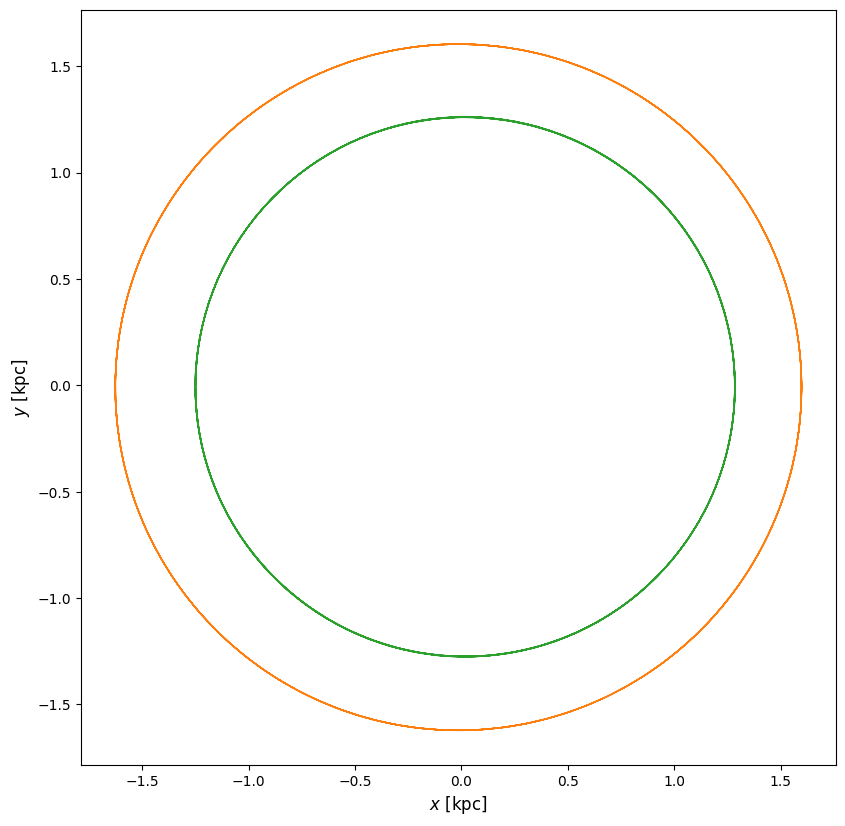
\includegraphics[scale=.50]{vip/normal.png}
    \caption{Orbit of galaxy when time step at 0.4 Myr}
    \label{fig:code}
\end{figure}
\begin{figure}[H]
    \centering
    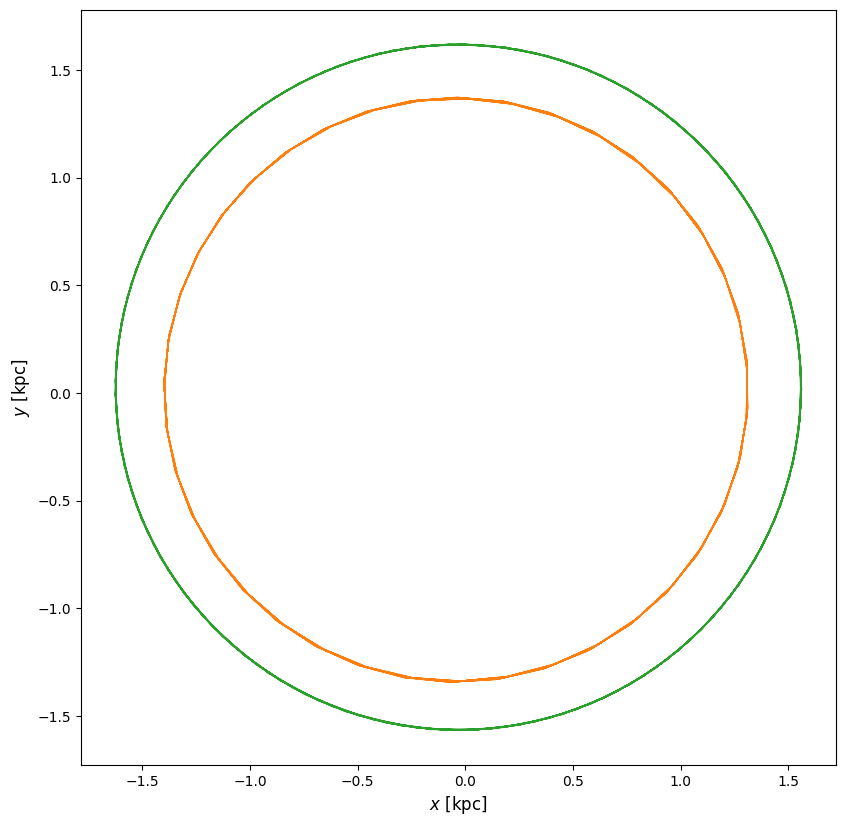
\includegraphics[scale=.50]{vip/0.6.png}
    \caption{Orbit of galaxy when time step at 0.6 Myr}
    \label{fig:code}
\end{figure}
\begin{figure}[H]
    \centering
    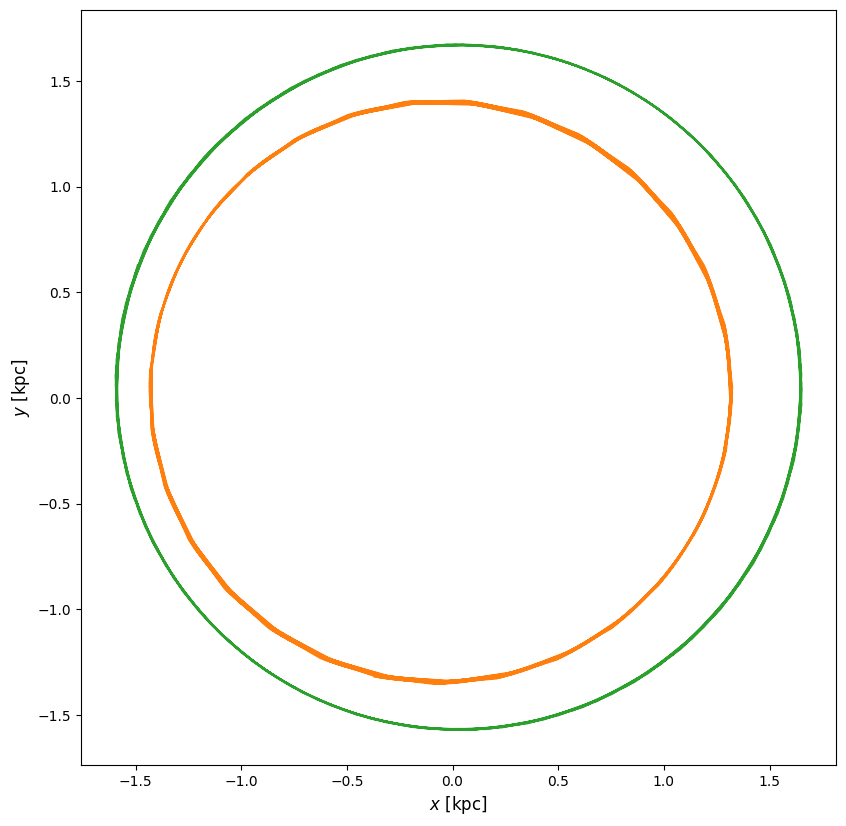
\includegraphics[scale=.50]{vip/0.8.png}
    \caption{Orbit of galaxy when time step at 0.8 Myr}
    \label{fig:code}
\end{figure}
\begin{figure}[H]
    \centering
    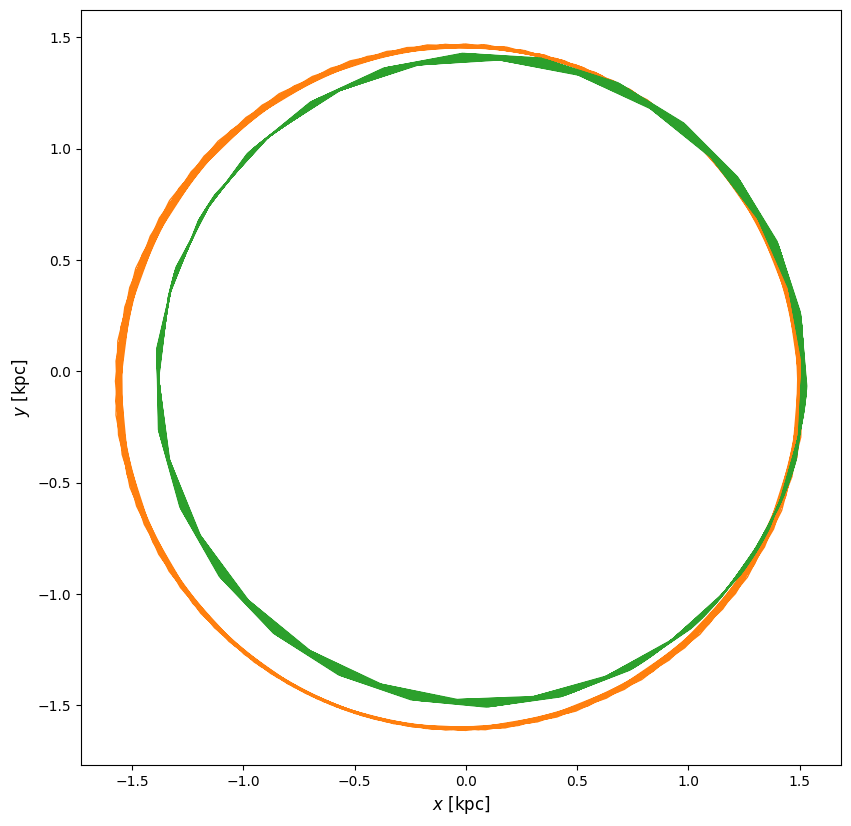
\includegraphics[scale=.50]{vip/1.png}
    \caption{Orbit of galaxy when time step at 1 Myr}
    \label{fig:code}
\end{figure}

Another observational phenomenon to note is the effect of the impact parameter, the ratio of the galaxies' velocity, the ratio of the galaxies' masses, and the relative angles of the galaxies. While running the investigations, the blue galaxy represents the target galaxy and the red galaxy represents the intruding galaxy.

When increasing the impact parameter (in kpc), the target galaxy retained more of its shape, showing that once the distance grows large enough, they begin to become less affected by each other. At 20 kpc, both galaxies missed each other and retained their respective shape, albeit the smaller galaxy was slightly affected by the larger galaxy's gravity. Below are images displaying the galaxies after a collision at different impact parameters.


The same could not be said when changing the relative velocities. The velocity of the intruding galaxy has been greater than the velocity of the target galaxy while changing the impact parameters. This has led to the previous observation of both galaxies starting to preserve their shape. The observation holds true if the impact parameter increases along with the target galaxy's velocity. However, once the velocity of the target galaxy increased at lower impact parameters, the intruding galaxy scatters more. Below are figures of when the velocity of the target galaxy is changed to be greater than the intruding galaxy.

\begin{figure}[H]
    \centering
    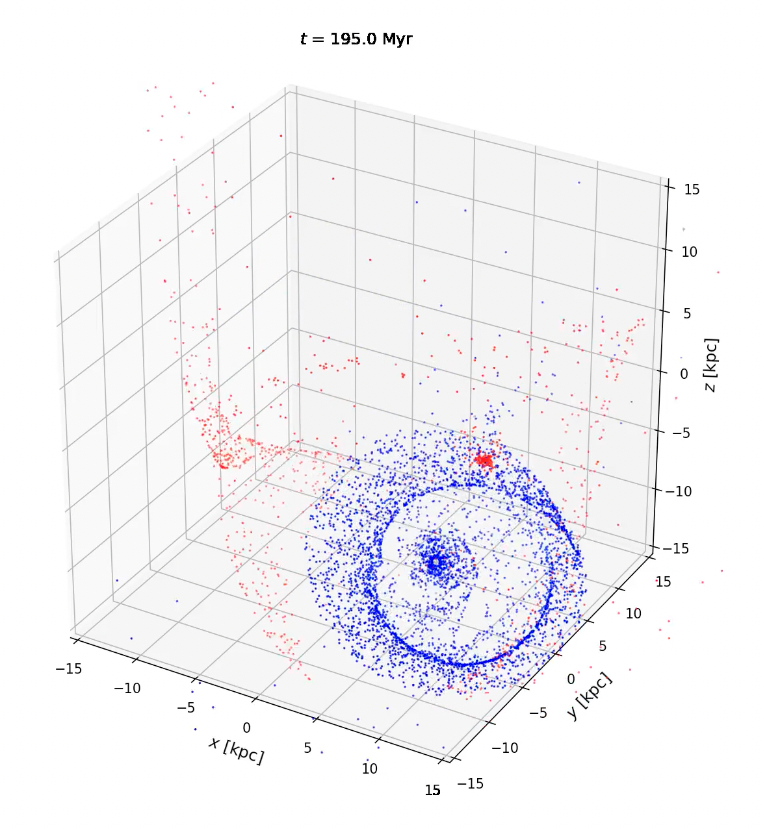
\includegraphics[scale=.40]{vip/b2targetv.png}
    \caption{Resulting galaxy when b = 2 and velocity of target galaxy is greater than intruding galaxy}
    \label{fig:code}
\end{figure}
\begin{figure}[H]
    \centering
    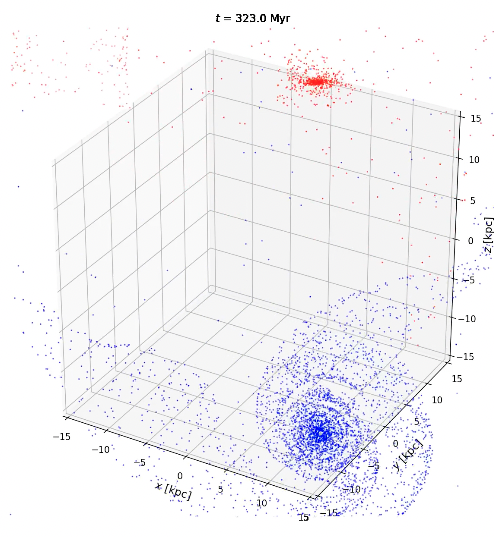
\includegraphics[scale=.50]{vip/b6equalv.png}
    \caption{Resulting galaxy when b = 6 and velocity of target galaxy is equal to intruding galaxy}
    \label{fig:code}
\end{figure}
\begin{figure}[H]
    \centering
    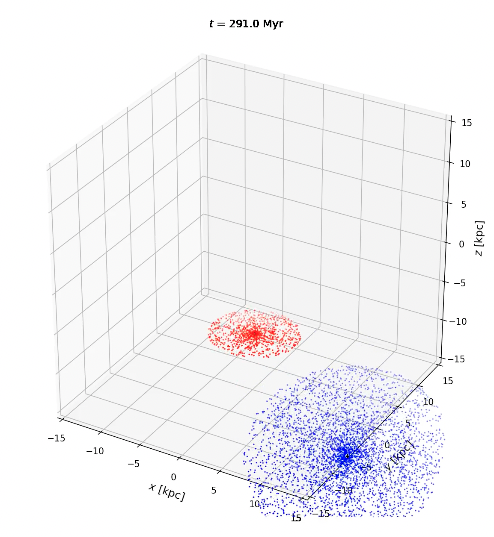
\includegraphics[scale=.50]{vip/b20targetv.png}
    \caption{Resulting galaxy when b = 20 and velocity of target galaxy is greater than intruding galaxy}
    \label{fig:code}
\end{figure}

Changing the ratio of the masses affects how the galaxies would look upon collision. The only variation in the ratio would be making the intruding galaxy's mass equal to the target galaxy or making the intruder mass much larger than the target mass. By making both galaxy's masses equal, they both shatter with their respective stars being strewn about while the centers rebound from each other. Making the intruder mass much larger than the target mass poses a similar scenario as when we make the velocity of the target galaxy much larger. What happens is that the target galaxy is the one being shattered, but this time, the center of the target galaxy is dragged along with the intruding galaxy. Below are figures depicting the end result of when the masses of both galaxies are equal.

\begin{figure}[H]
    \centering
    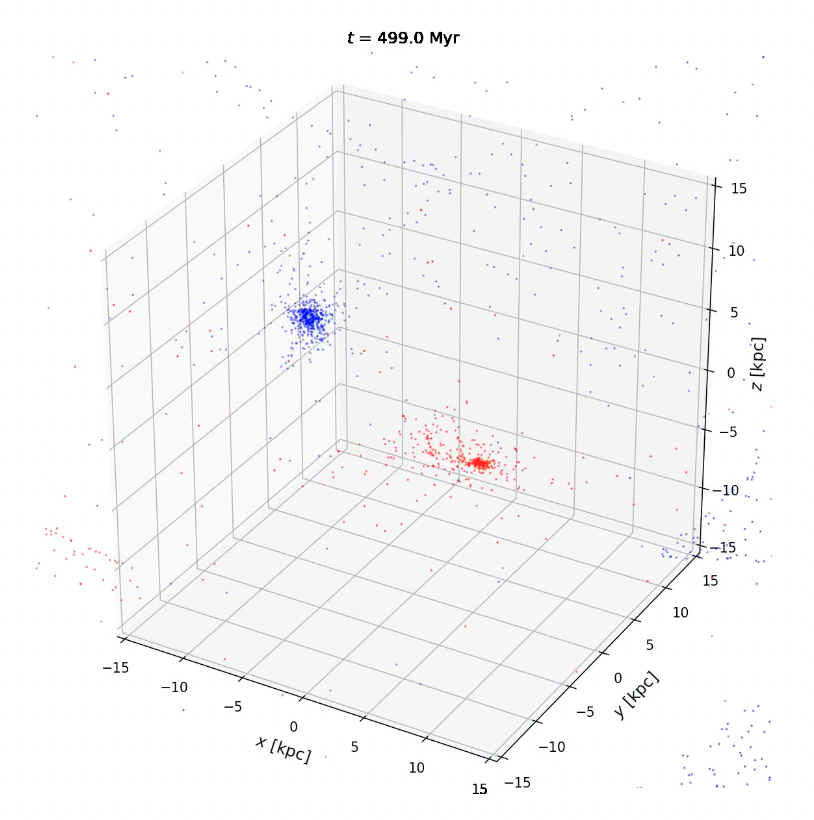
\includegraphics[scale=.50]{vip/b6equalmass.png}
    \caption{Resulting galaxy when b = 2 and the masses of both galaxies are equal}
    \label{fig:code}
\end{figure}
\begin{figure}[H]
    \centering
    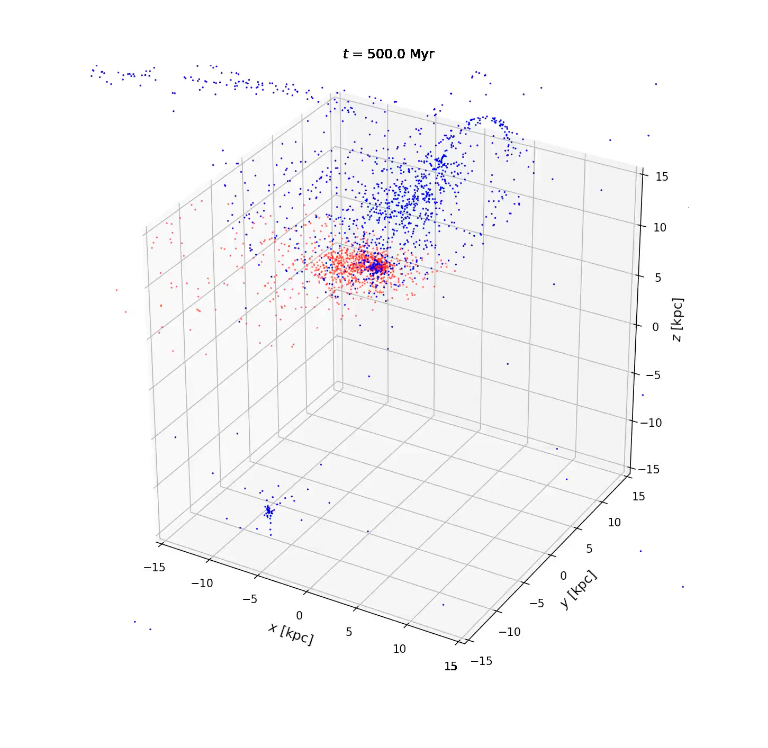
\includegraphics[scale=.50]{vip/b6intrudermass.png}
    \caption{Resulting galaxy when b = 6 and the intruding mass is greater than the target}
    \label{fig:code}
\end{figure}

When adjusting the orientation of the target galaxy, the resulting galaxies are similar to each other. Here, the angle was manipulated along the zx plane. The intruding galaxy veers to the upper right while the target galaxy resembles a spiral pattern. The only differences between the variation of angles is the orientation of the resulting galaxies and that as the angles become closer to $90^{\circ}$, more stars can be observed to be scatter along the z and x plane. Below are figures that depict the resulting galaxies at different angles. 

\begin{figure}[H]
    \centering
    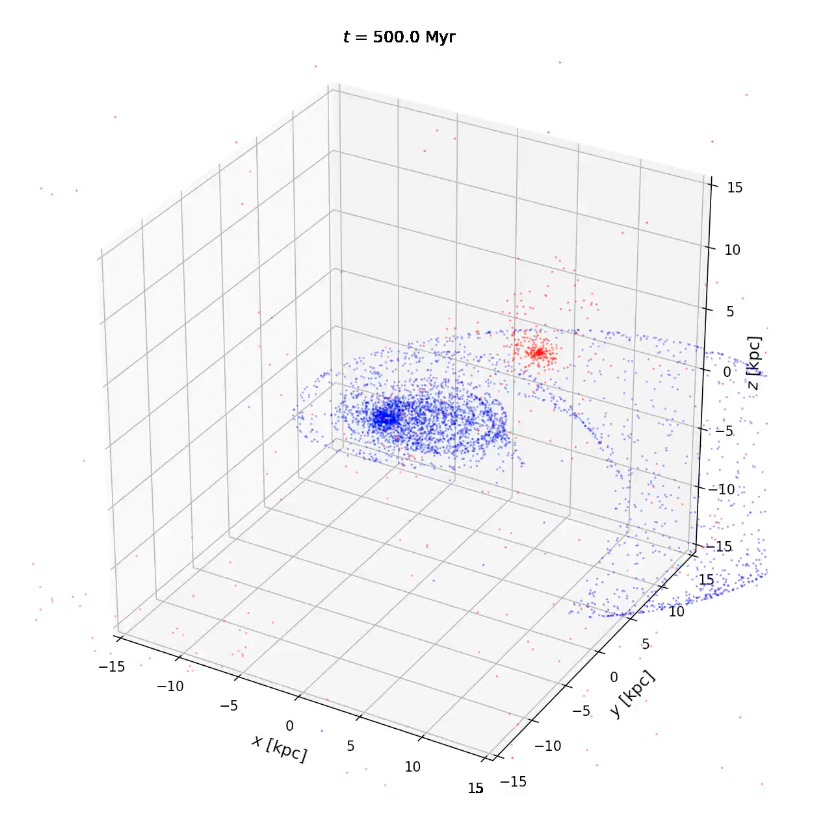
\includegraphics[scale=.50]{vip/0ngle.png}
    \caption{Resulting galaxy when the angle of the target galaxy is 0 degrees}
    \label{fig:code}
\end{figure}
\begin{figure}[H]
    \centering
    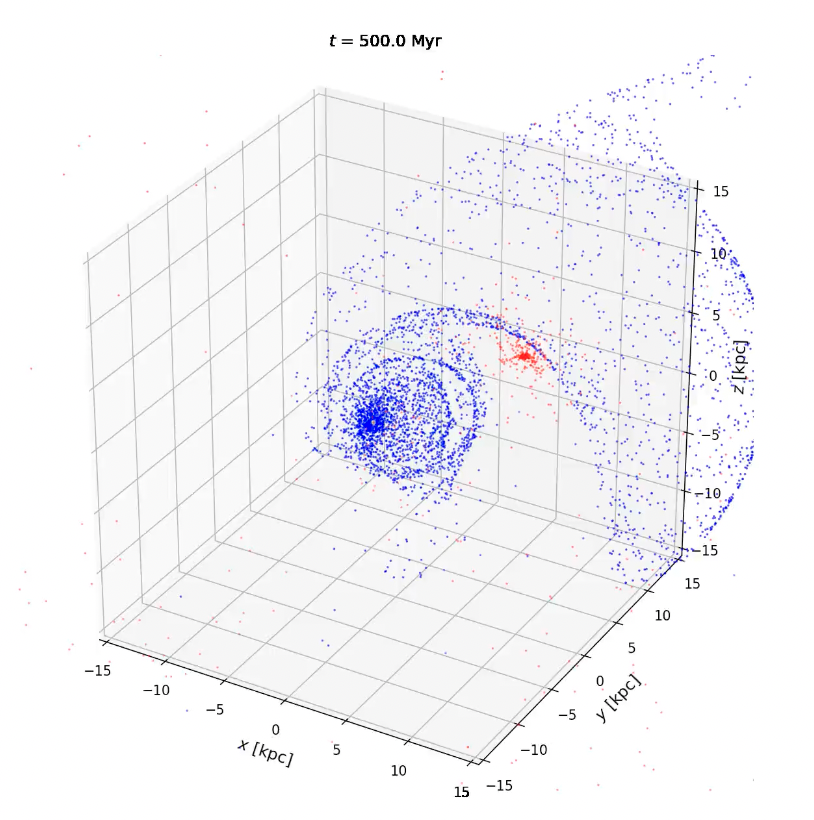
\includegraphics[scale=.50]{vip/45angle.png}
    \caption{Resulting galaxy when the angle of the target galaxy is 45 degrees}
    \label{fig:code}
\end{figure}
\begin{figure}[H]
    \centering
    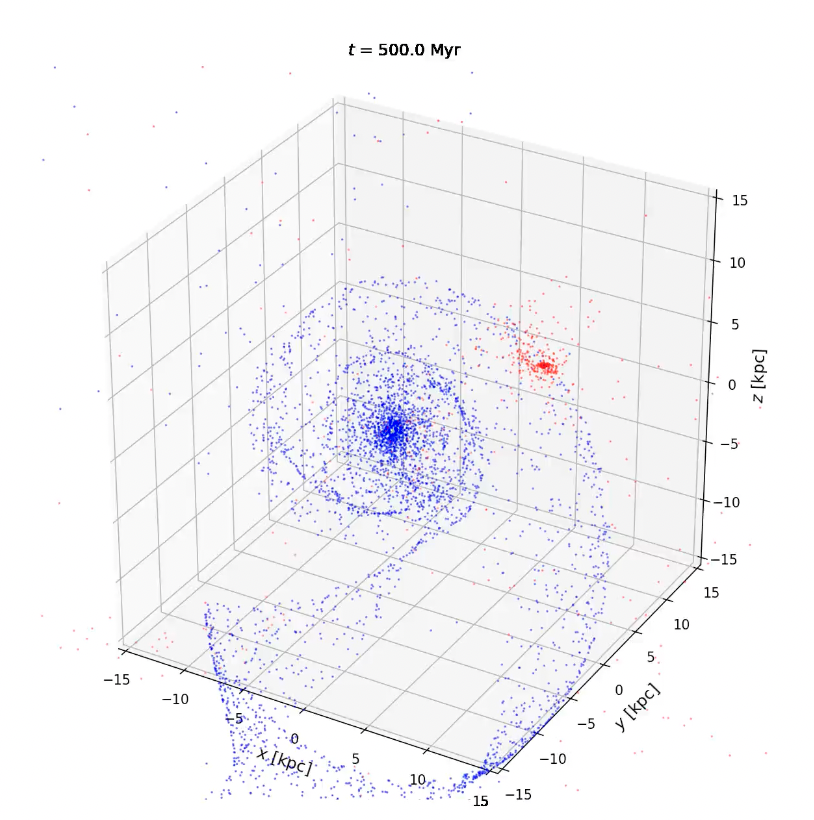
\includegraphics[scale=.50]{vip/65.9angle.png}
    \caption{Resulting galaxy when the angle of the target galaxy is 65.9 degrees}
    \label{fig:code}
\end{figure}
\begin{figure}[H]
    \centering
    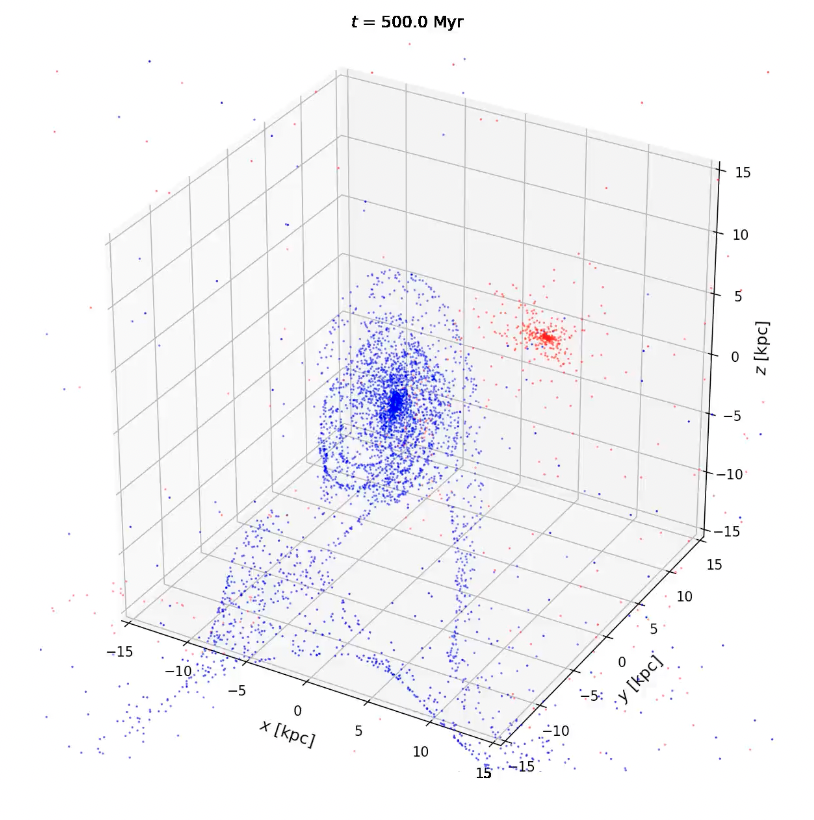
\includegraphics[scale=.50]{vip/90angle.png}
    \caption{Resulting galaxy when the angle of the target galaxy is 90 degrees}
    \label{fig:code}
\end{figure}

\section{Comparison} \label{sec:method}
The velocity of a galaxy was adjusted to recreate a cartwheel galaxy using the simulation. The galaxies were placed at the same x and y coordinates, but with a different z coordinate. The intruding galaxy was placed with a negative z coordinate, whereas the intruded galaxy had a positive z coordinate. The normal of the intruding galaxy is in the same direction as the velocity: in the positive z direction. The results are shown below.

% Cartwheel galaxy
\begin{figure}[H]
    \centering
    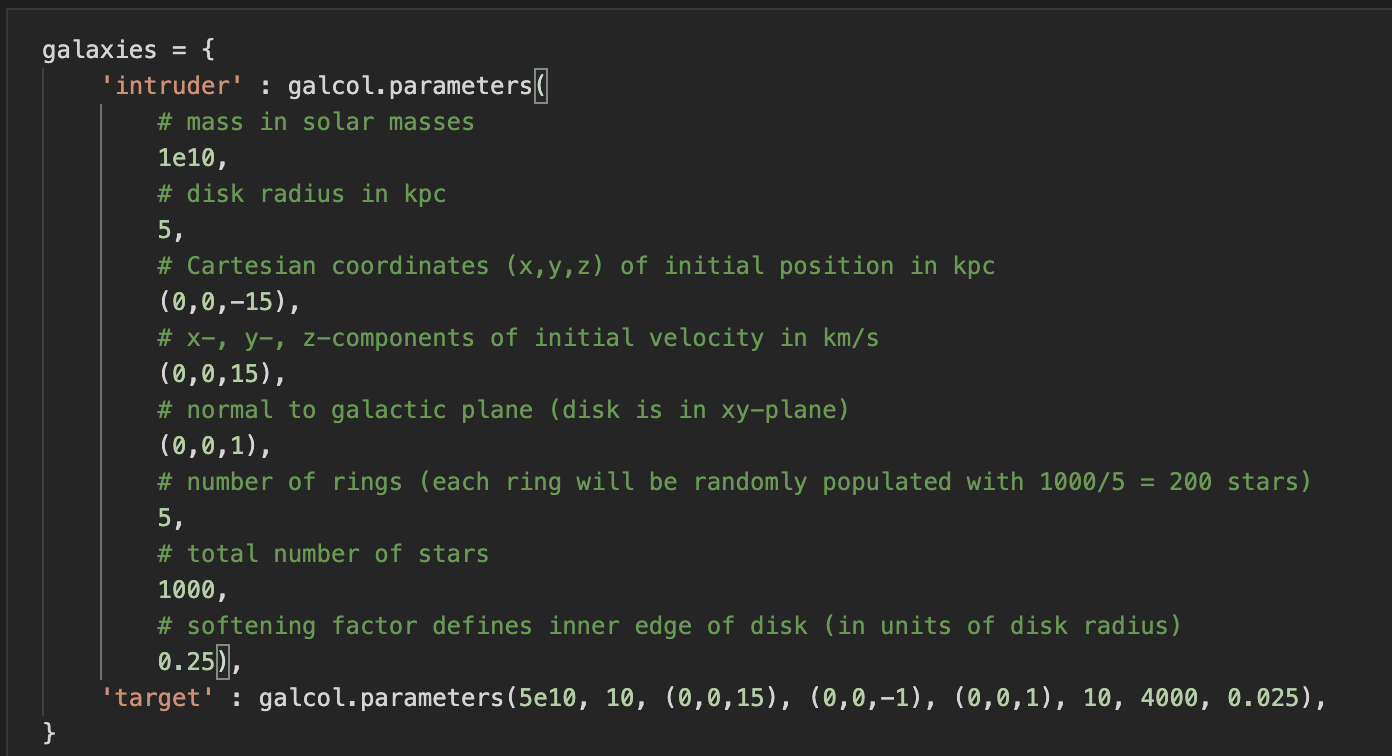
\includegraphics[scale=.70]{cartwheel_input_vars.png}
    \caption{The velocity of the intruder is 15 km/s in the z direction}
    \label{fig:code}
\end{figure}
\newpage
\begin{figure}[H]
    \centering
    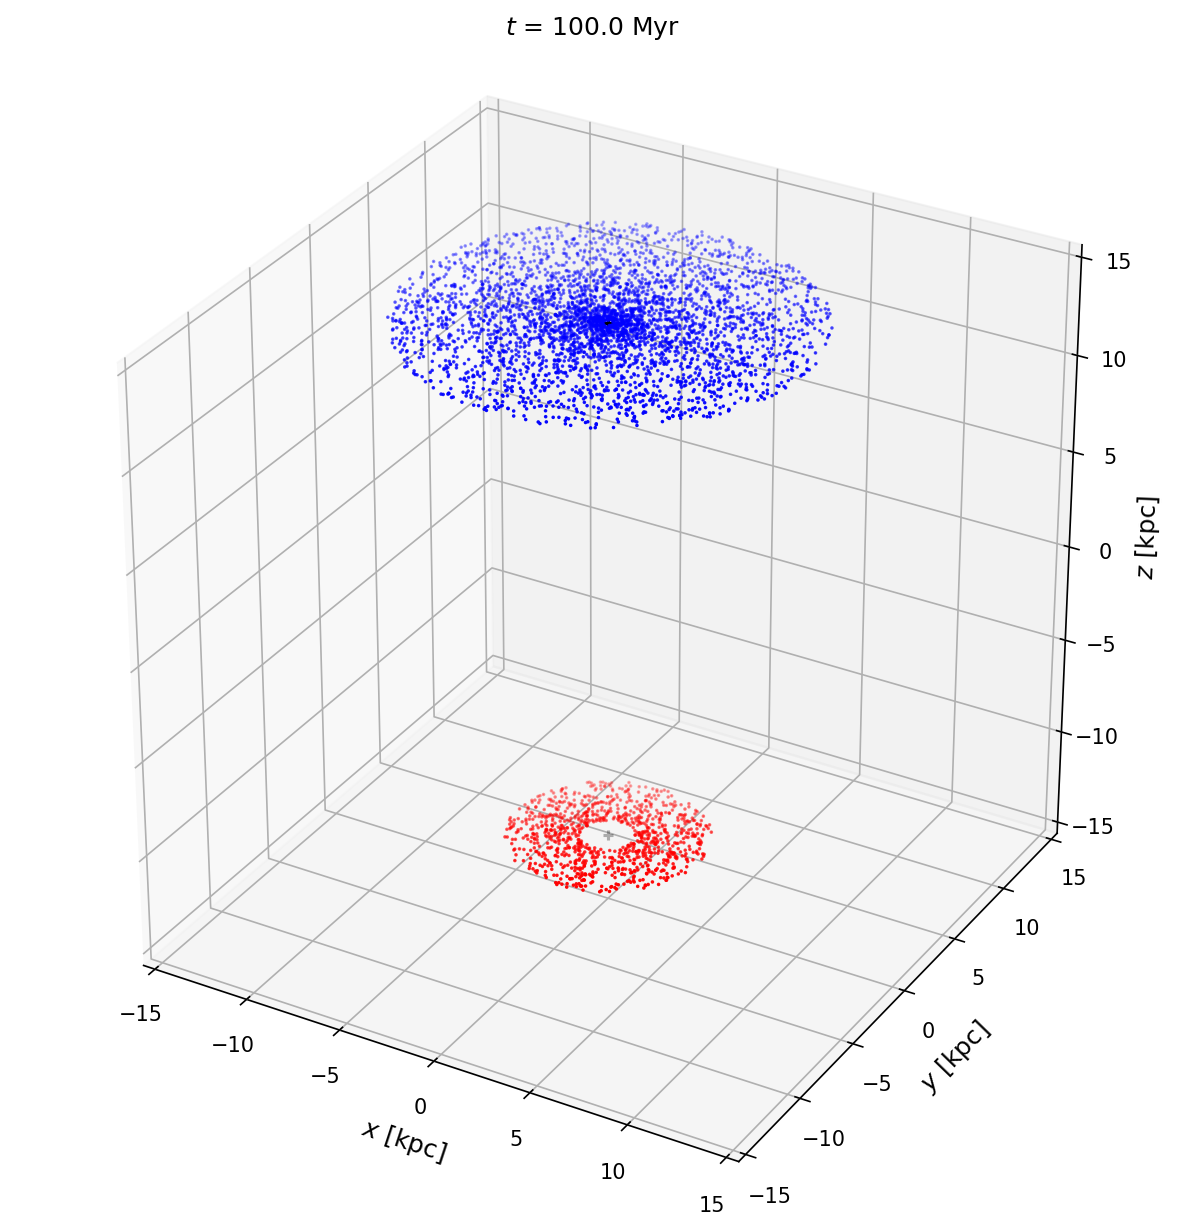
\includegraphics[scale=.40]{cartwheel_input.png}
    \caption{Start}
    \label{fig:code}
\end{figure}
\begin{figure}[H]
    \centering
    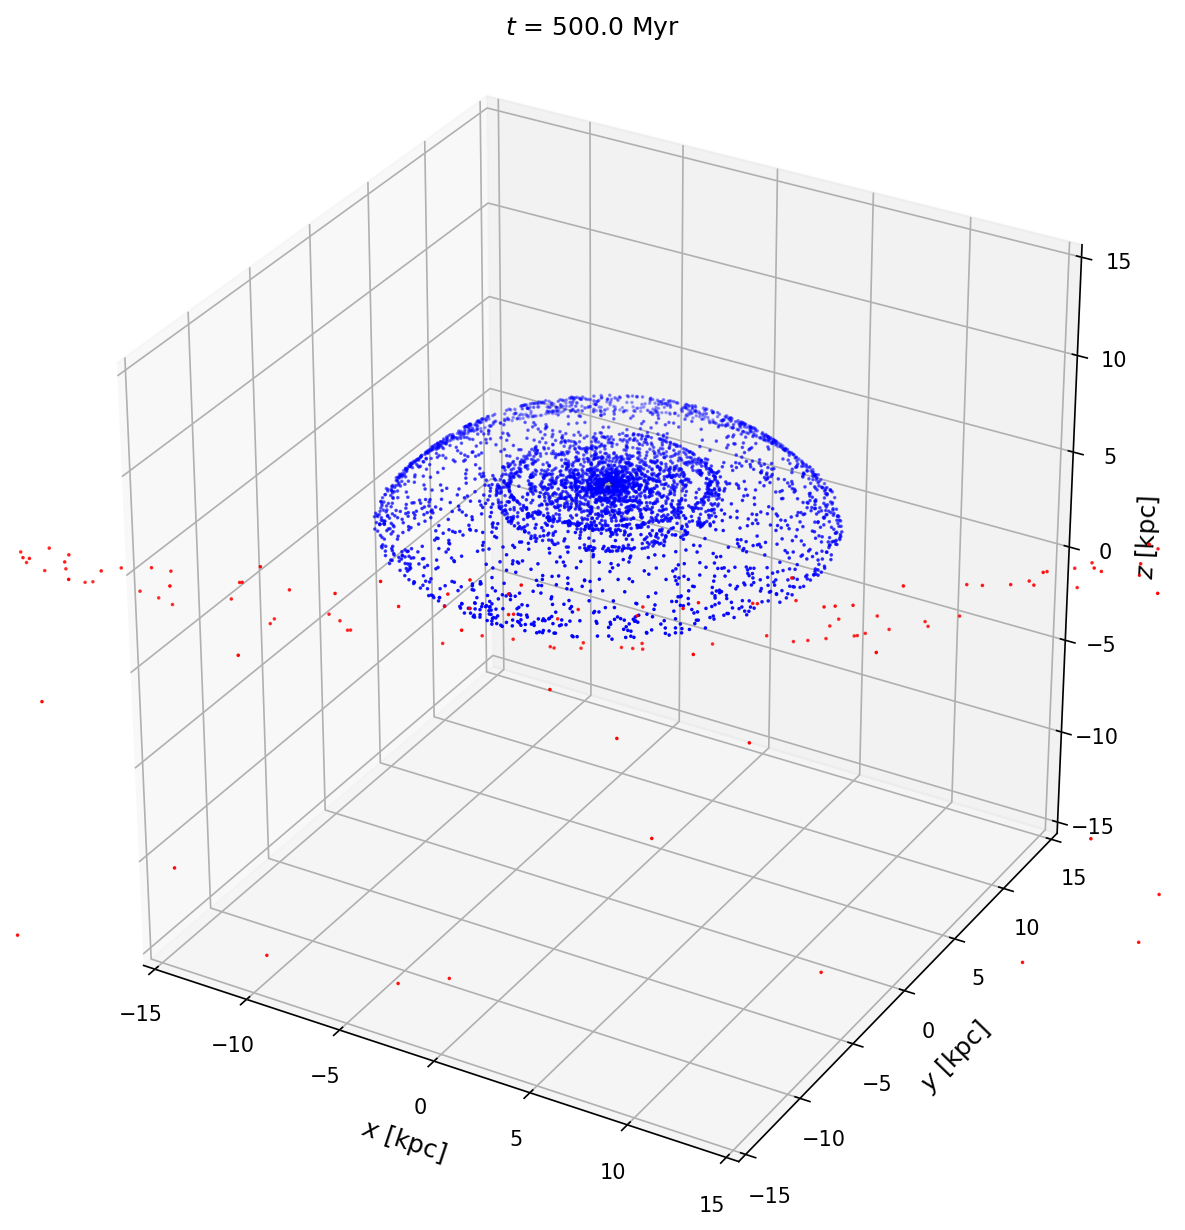
\includegraphics[scale=.40]{cartwheel.png}
    \caption{Finish}
    \label{fig:code}
\end{figure}
\begin{figure}[H]
    \centering
    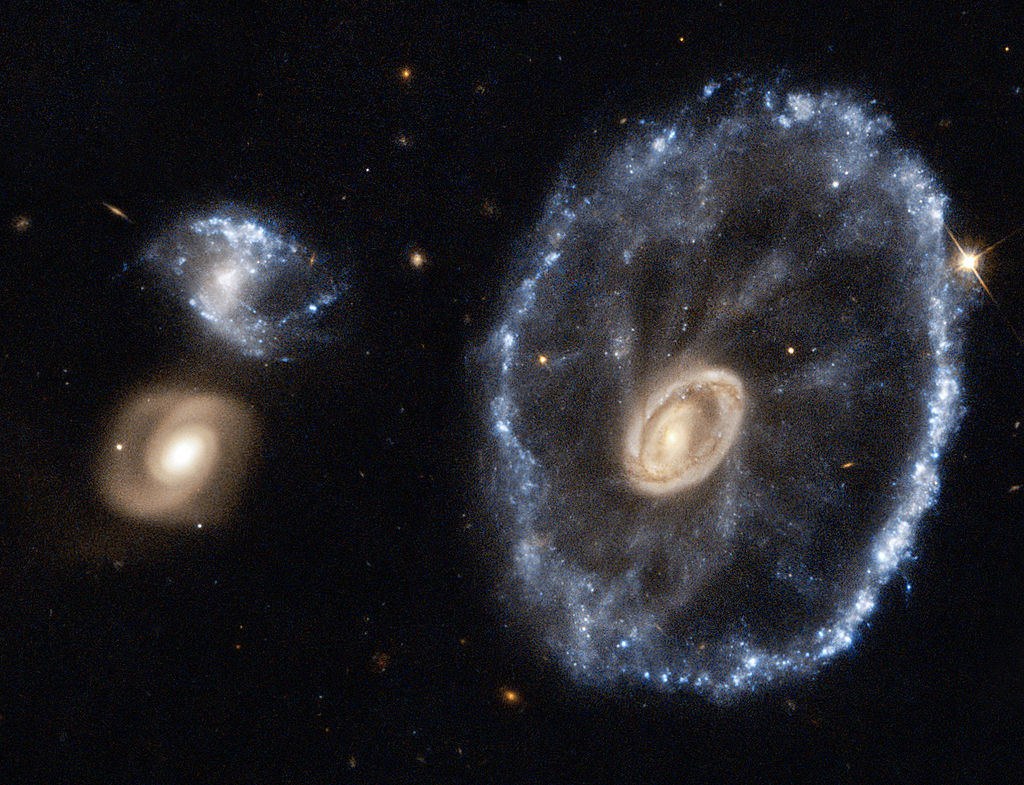
\includegraphics[scale=.5]{cartwheel.jpeg}
    \caption{Cartwheel Galaxy}
    \label{fig:code}
\end{figure}



\newpage
Varying the velocity and angles of the galaxies produces different outputs which can be compared to images from the Atlas of Peculiar Galaxies by Halton Arp. \cite{Arp}
% E1
\begin{figure}[H]
    \centering
    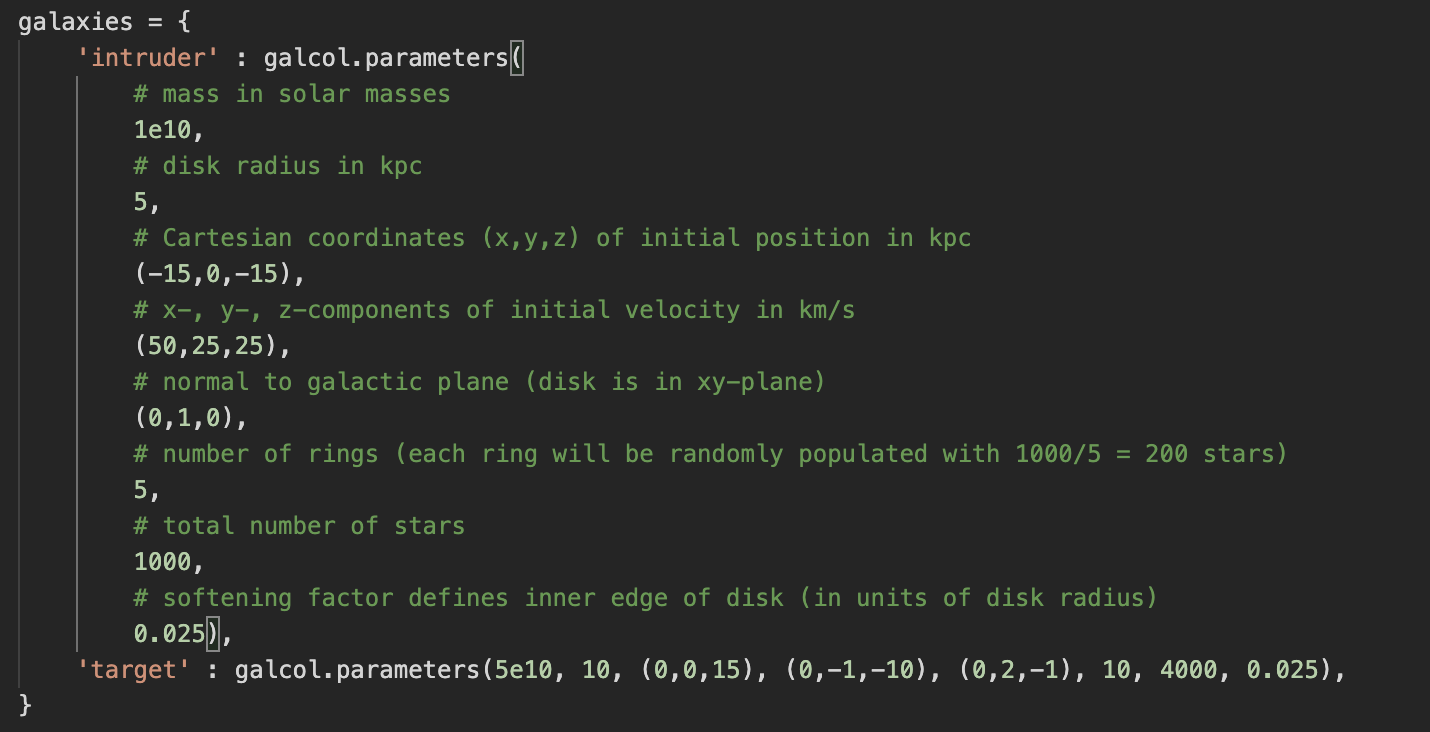
\includegraphics[scale=.60]{comparison_galaxy/ARP_9_vars.png}
    \caption{Varying position, velocity, and normal}
    \label{fig:code}
\end{figure}
\newpage
\begin{figure}[H]
    \centering
    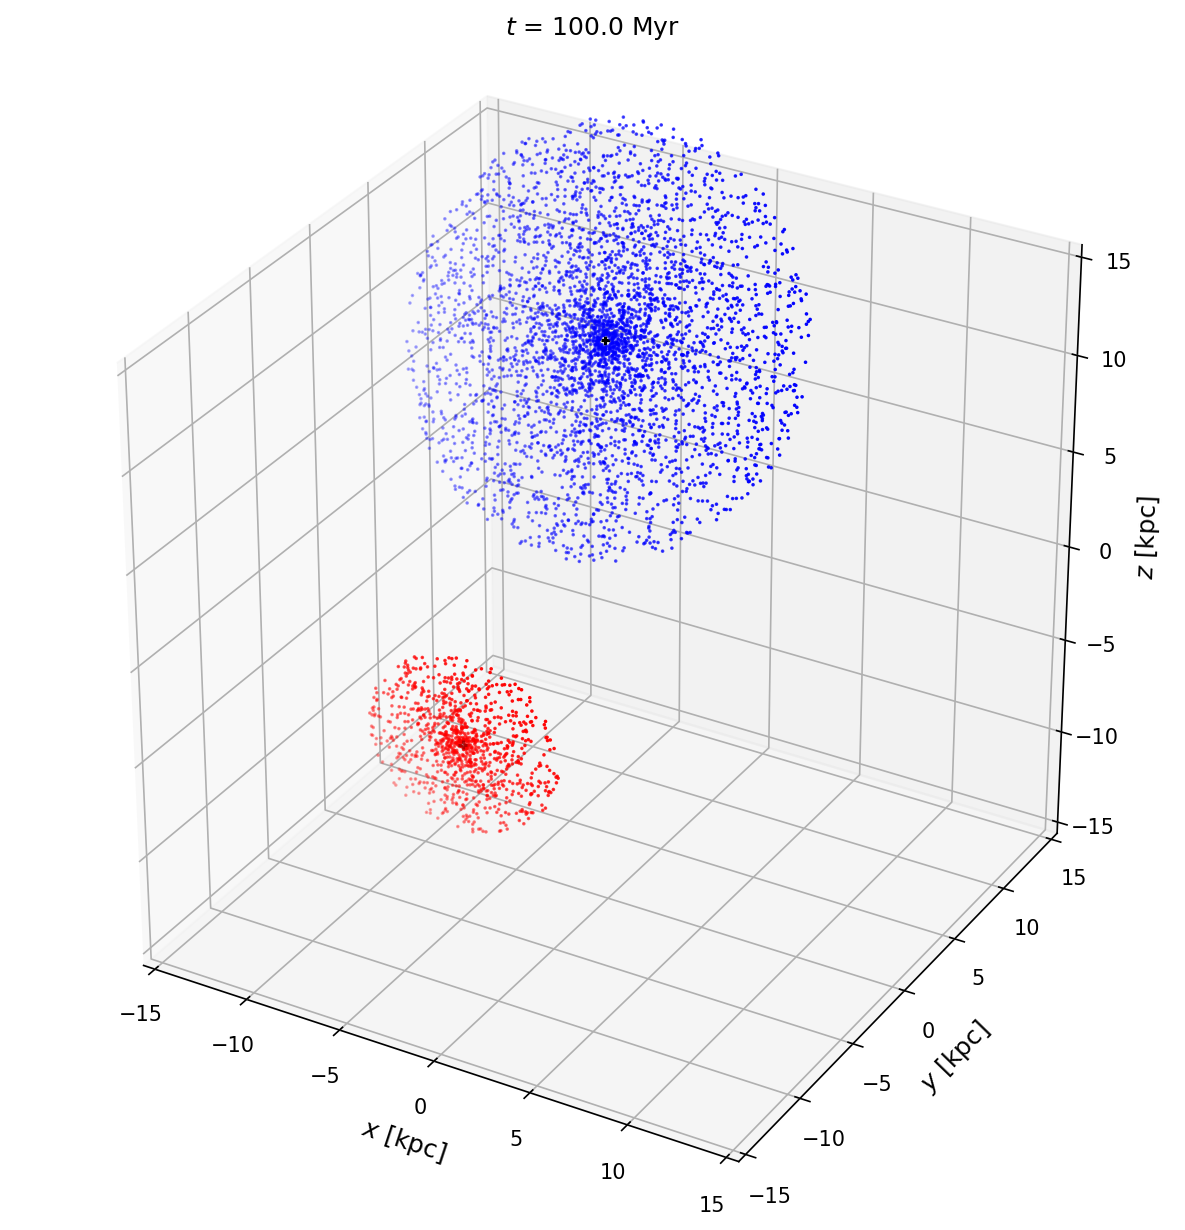
\includegraphics[scale=.40]{comparison_galaxy/ARP_9_input.png}
    \caption{Start}
    \label{fig:code}
\end{figure}
\begin{figure}[H]
    \centering
    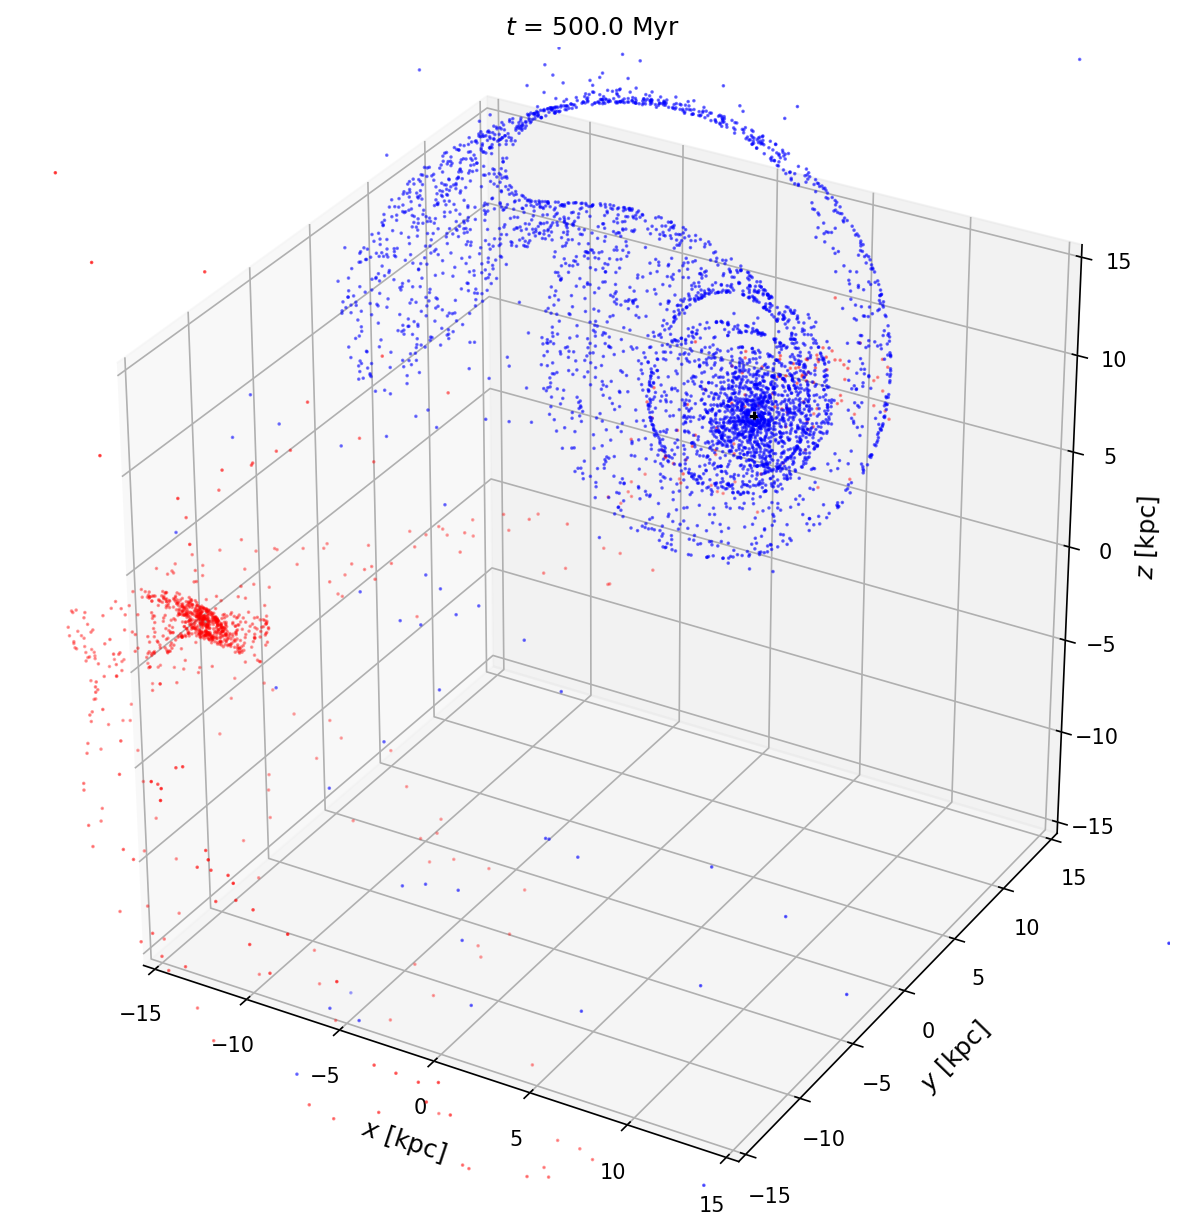
\includegraphics[scale=.40]{comparison_galaxy/ARP_9_output.png}
    \caption{Finish}
    \label{fig:code}
\end{figure}
\begin{figure}[H]
    \centering
    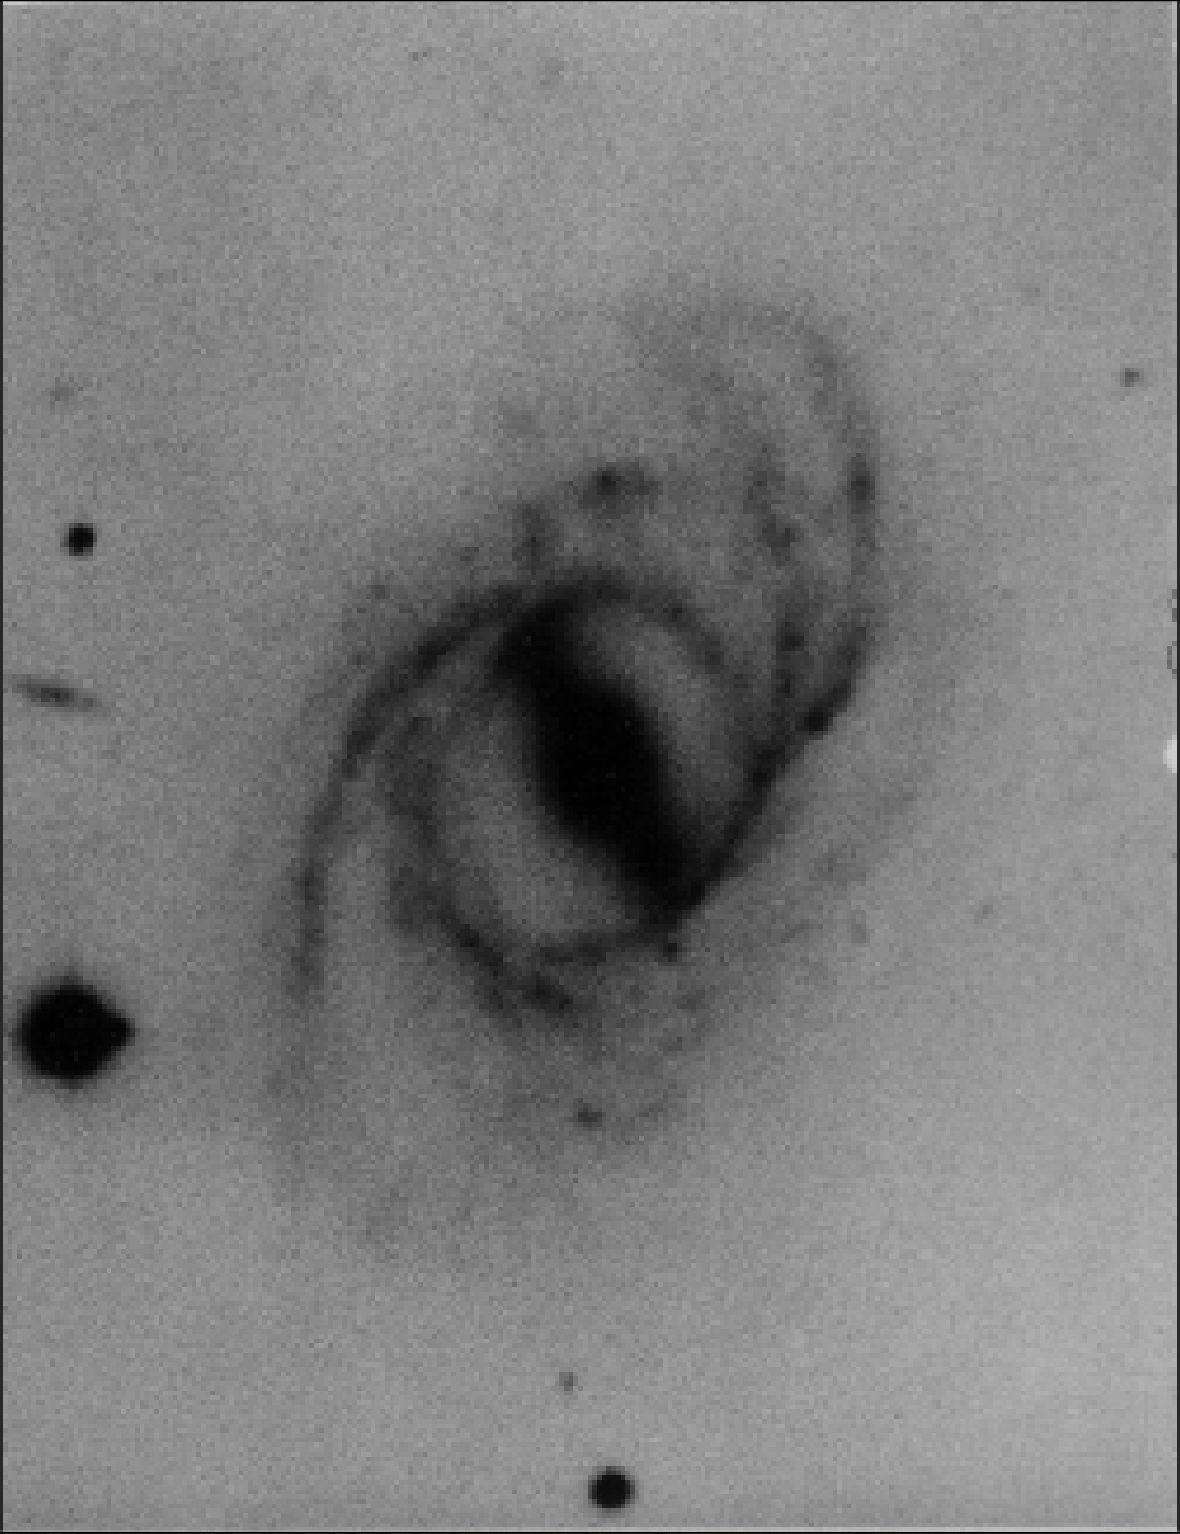
\includegraphics[scale=.50]{comparison_galaxy/arp_9.png}
    \caption{From Atlas Of Peculiar Galaxies, ARP 9}
    \label{fig:code}
\end{figure}





% E2
\begin{figure}[H]
    \centering
    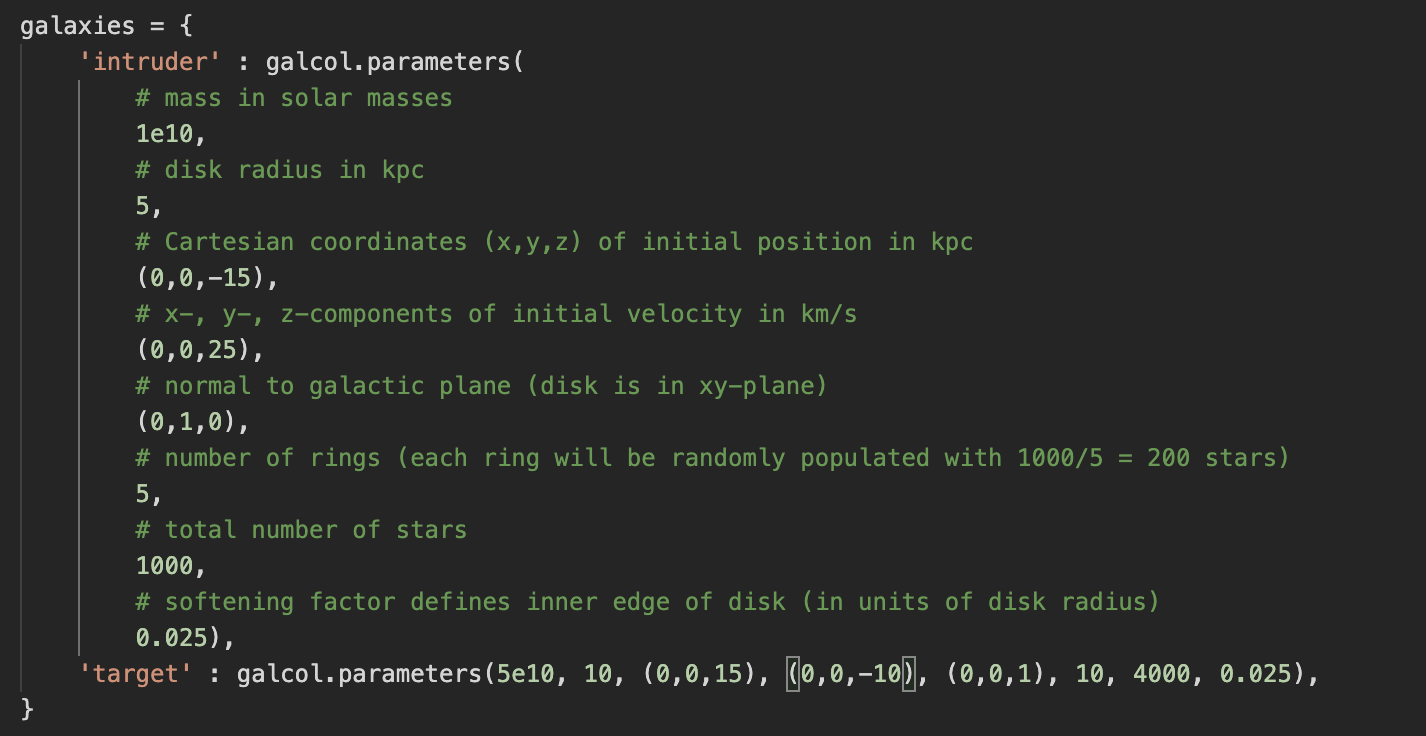
\includegraphics[scale=.60]{comparison_galaxy/ARP_10_vars.png}
    \caption{Varying position, velocity, and normal}
    \label{fig:code}
\end{figure}
\newpage
\begin{figure}[H]
    \centering
    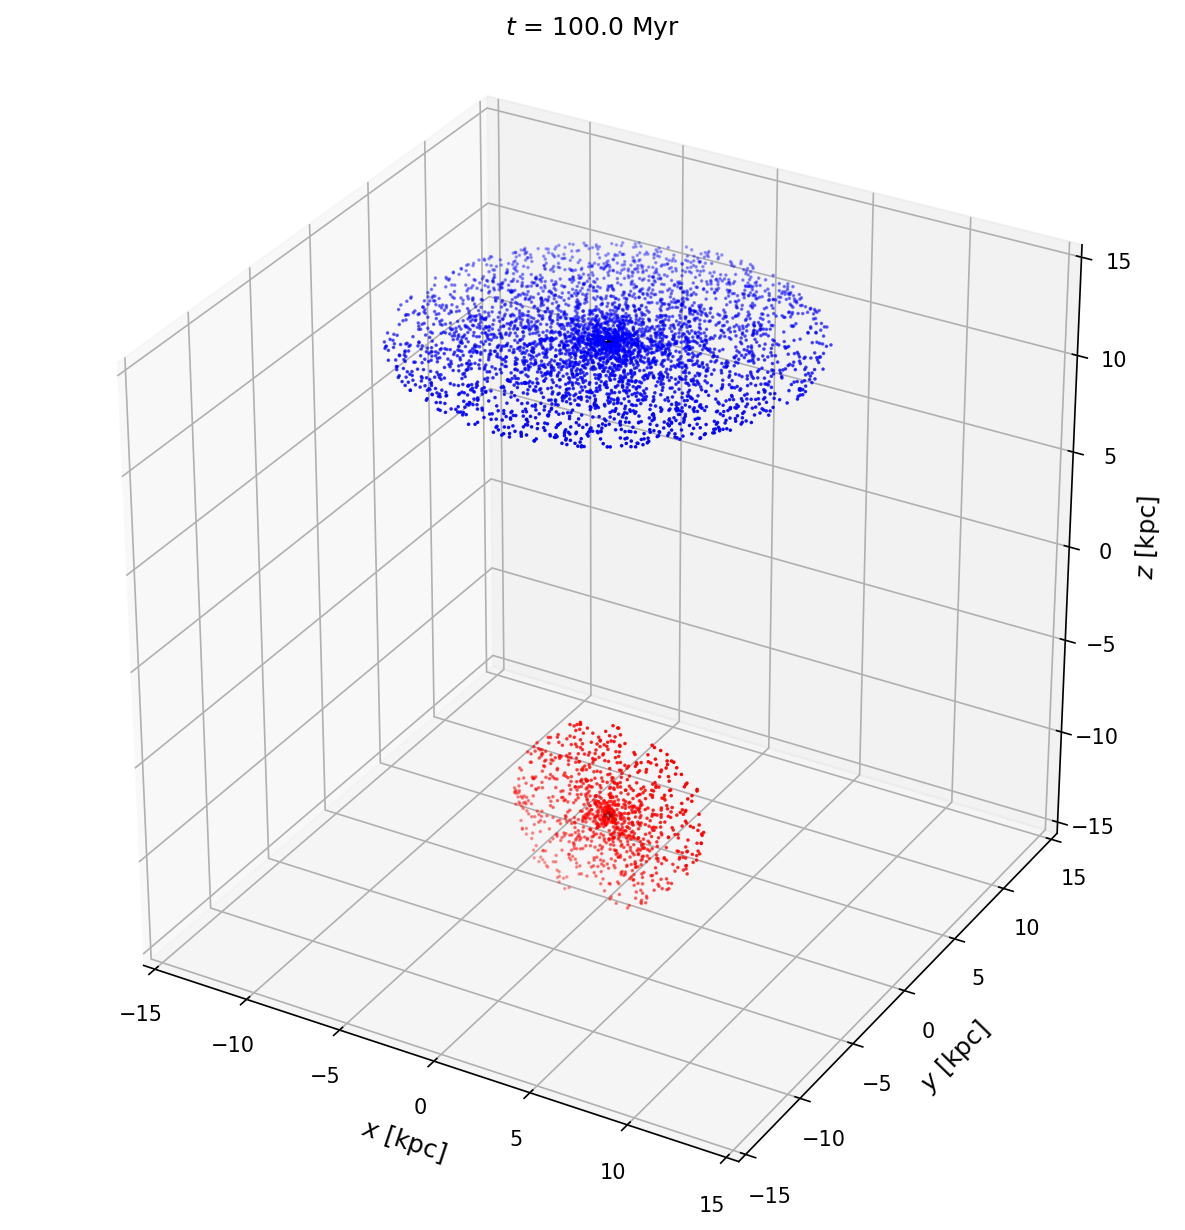
\includegraphics[scale=.40]{comparison_galaxy/ARP_10_input.png}
    \caption{Start}
    \label{fig:code}
\end{figure}
\begin{figure}[H]
    \centering
    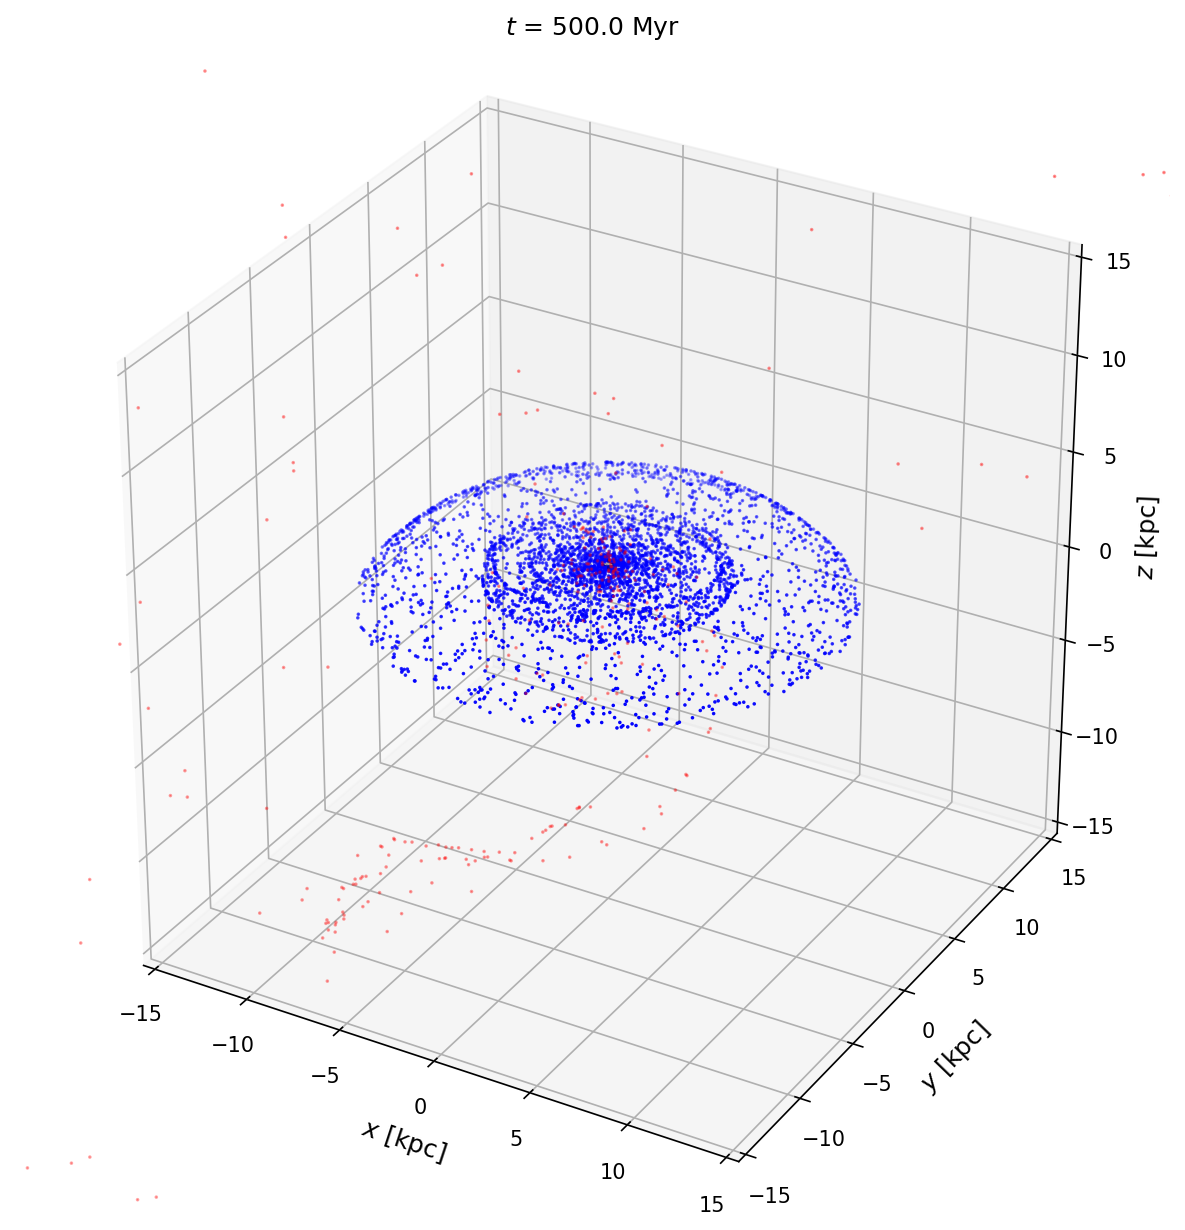
\includegraphics[scale=.40]{comparison_galaxy/ARP_10_output.png}
    \caption{Finish}
    \label{fig:code}
\end{figure}
\begin{figure}[H]
    \centering
    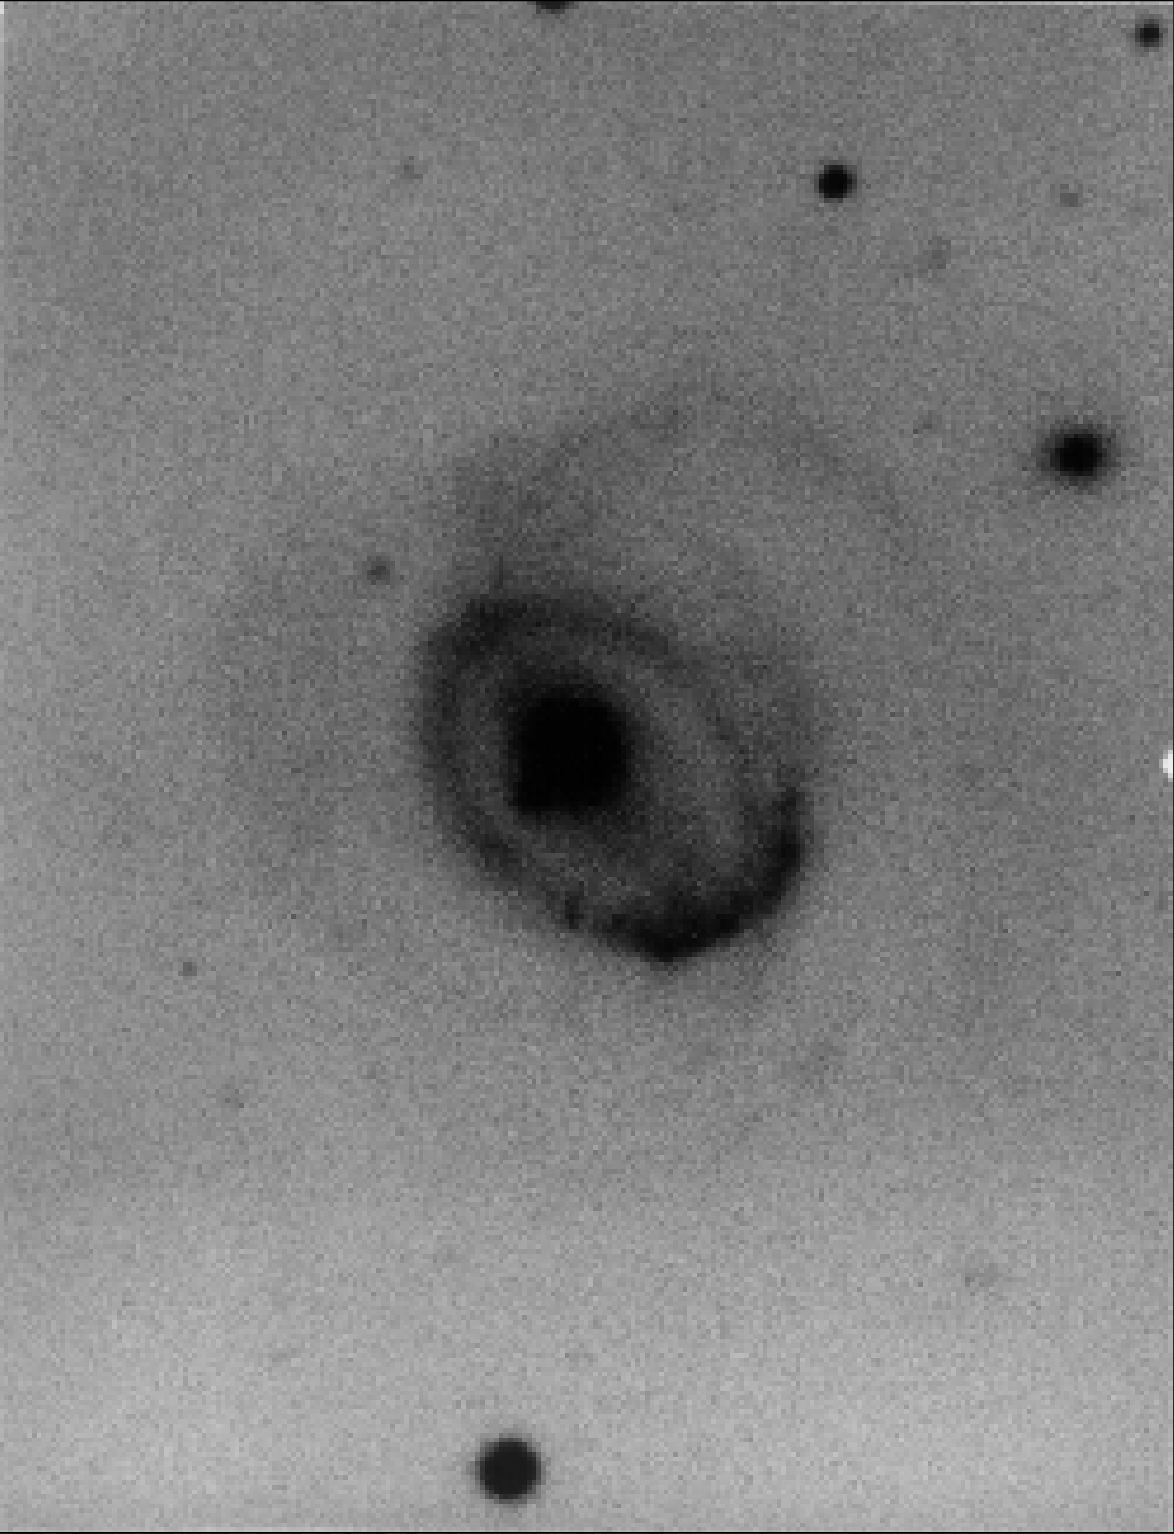
\includegraphics[scale=.50]{comparison_galaxy/arp_10.png}
    \caption{From Atlas Of Peculiar Galaxies, ARP 10}
    \label{fig:code}
\end{figure}





% E3
\begin{figure}[H]
    \centering
    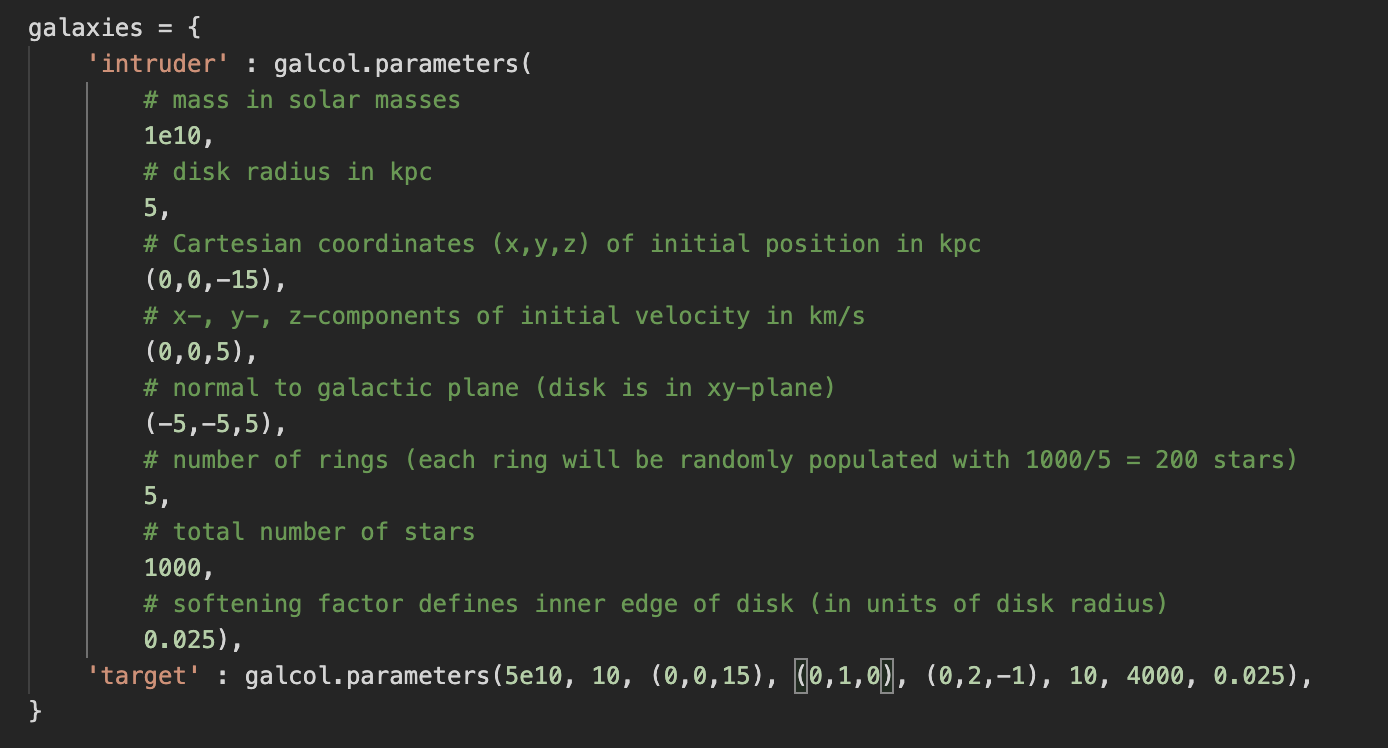
\includegraphics[scale=.60]{comparison_galaxy/ARP_42_vars.png}
    \caption{Varying position, velocity, and normal}
    \label{fig:code}
\end{figure}
\newpage
\begin{figure}[H]
    \centering
    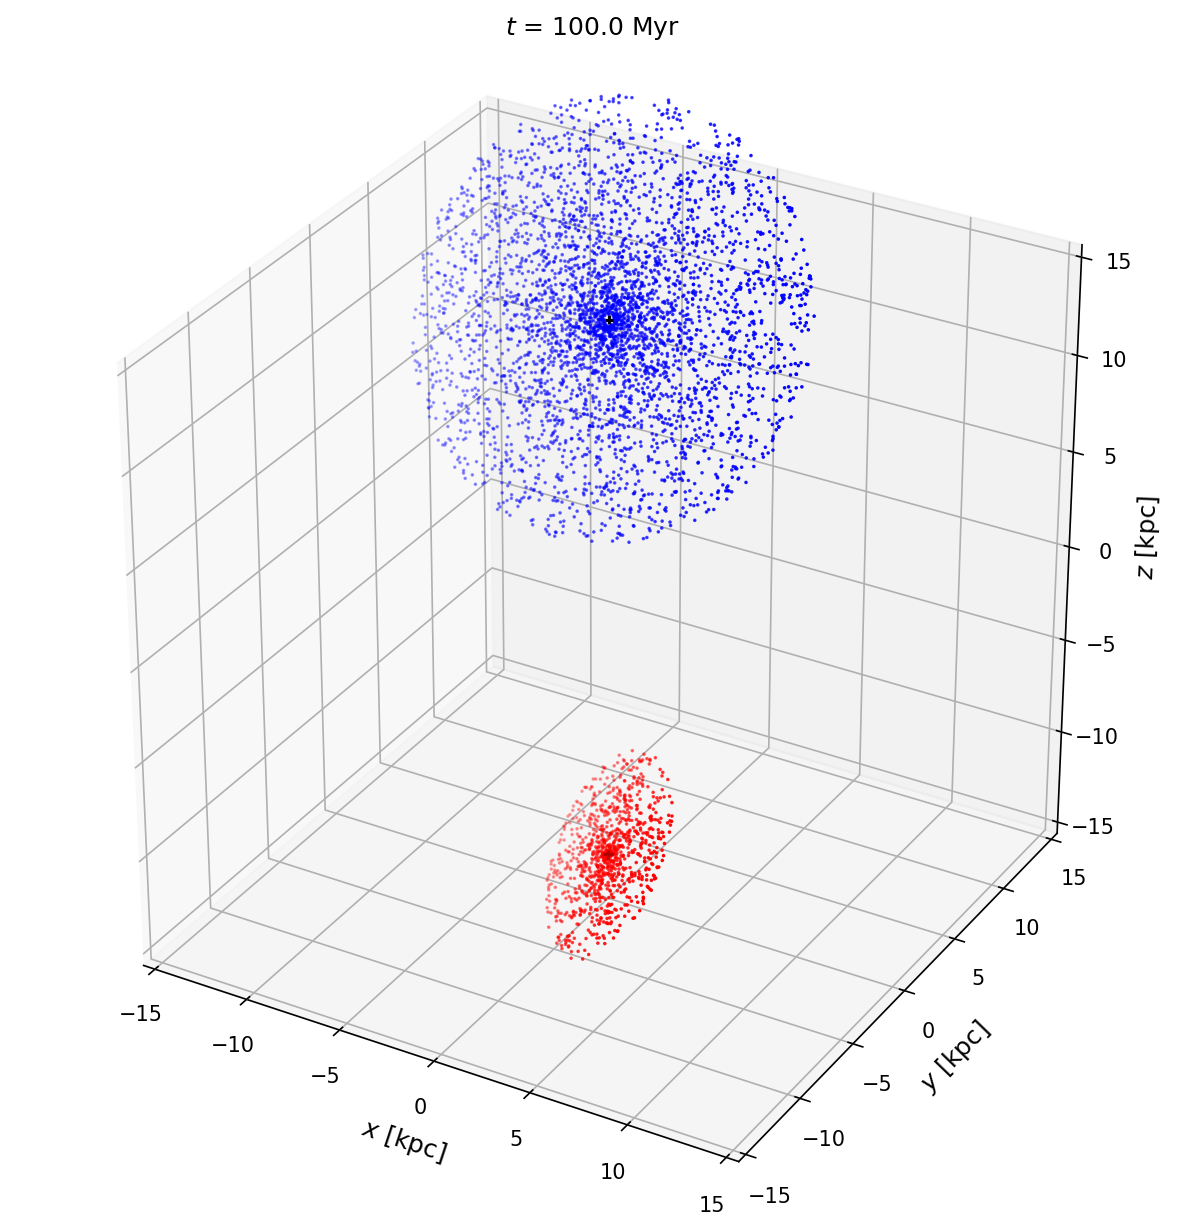
\includegraphics[scale=.40]{comparison_galaxy/ARP_42_input.png}
    \caption{Start}
    \label{fig:code}
\end{figure}
\begin{figure}[H]
    \centering
    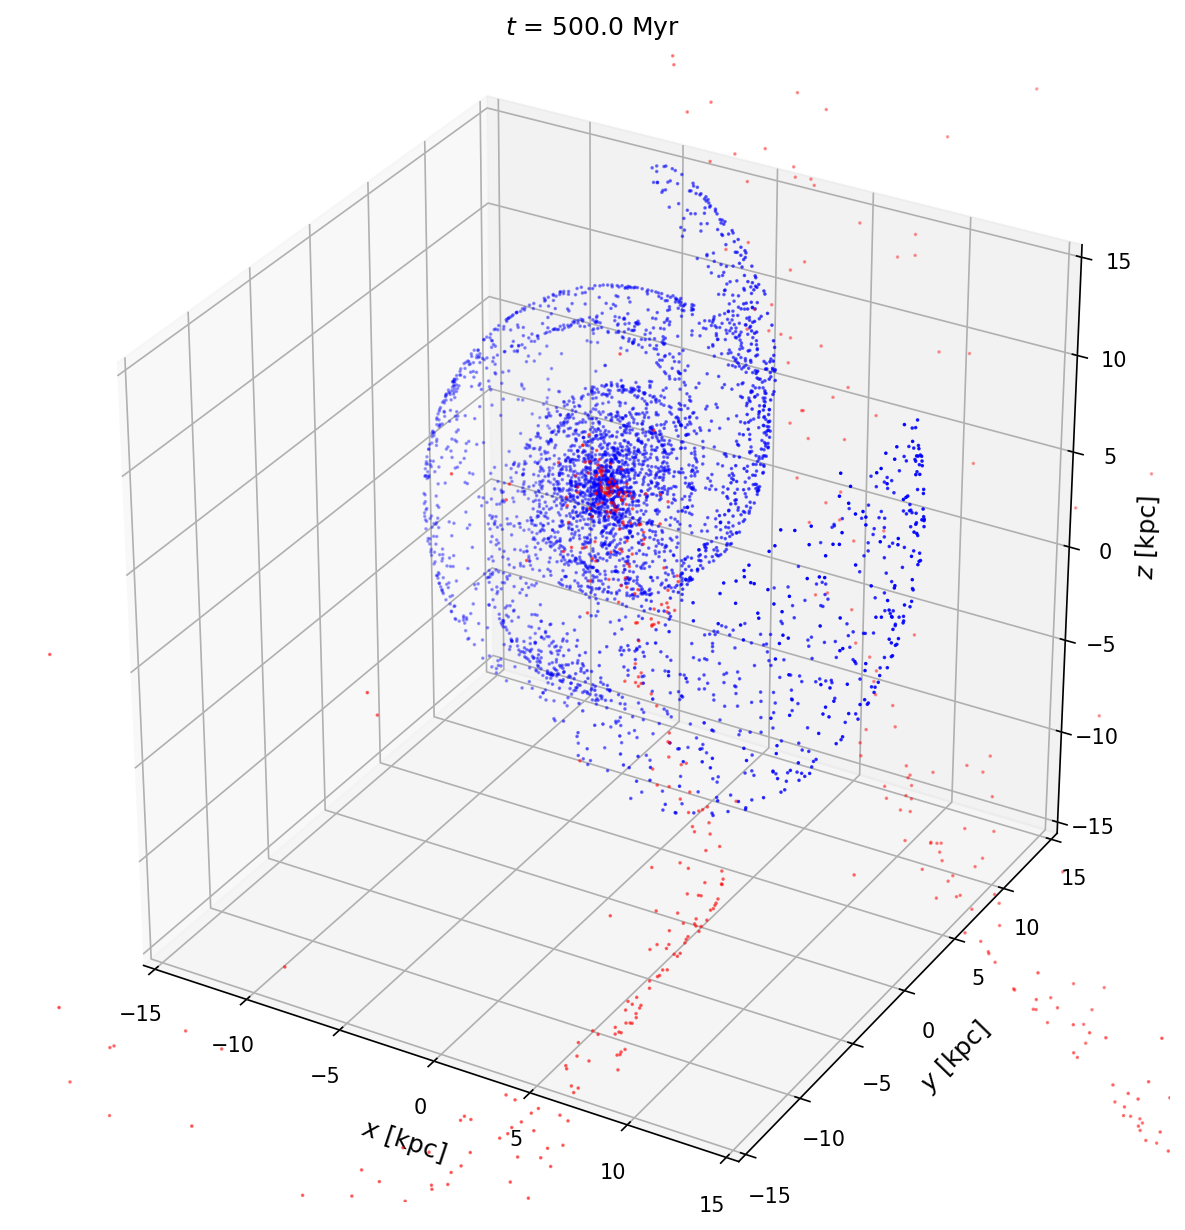
\includegraphics[scale=.40]{comparison_galaxy/ARP_42_output.png}
    \caption{Finish}
    \label{fig:code}
\end{figure}
\begin{figure}[H]
    \centering
    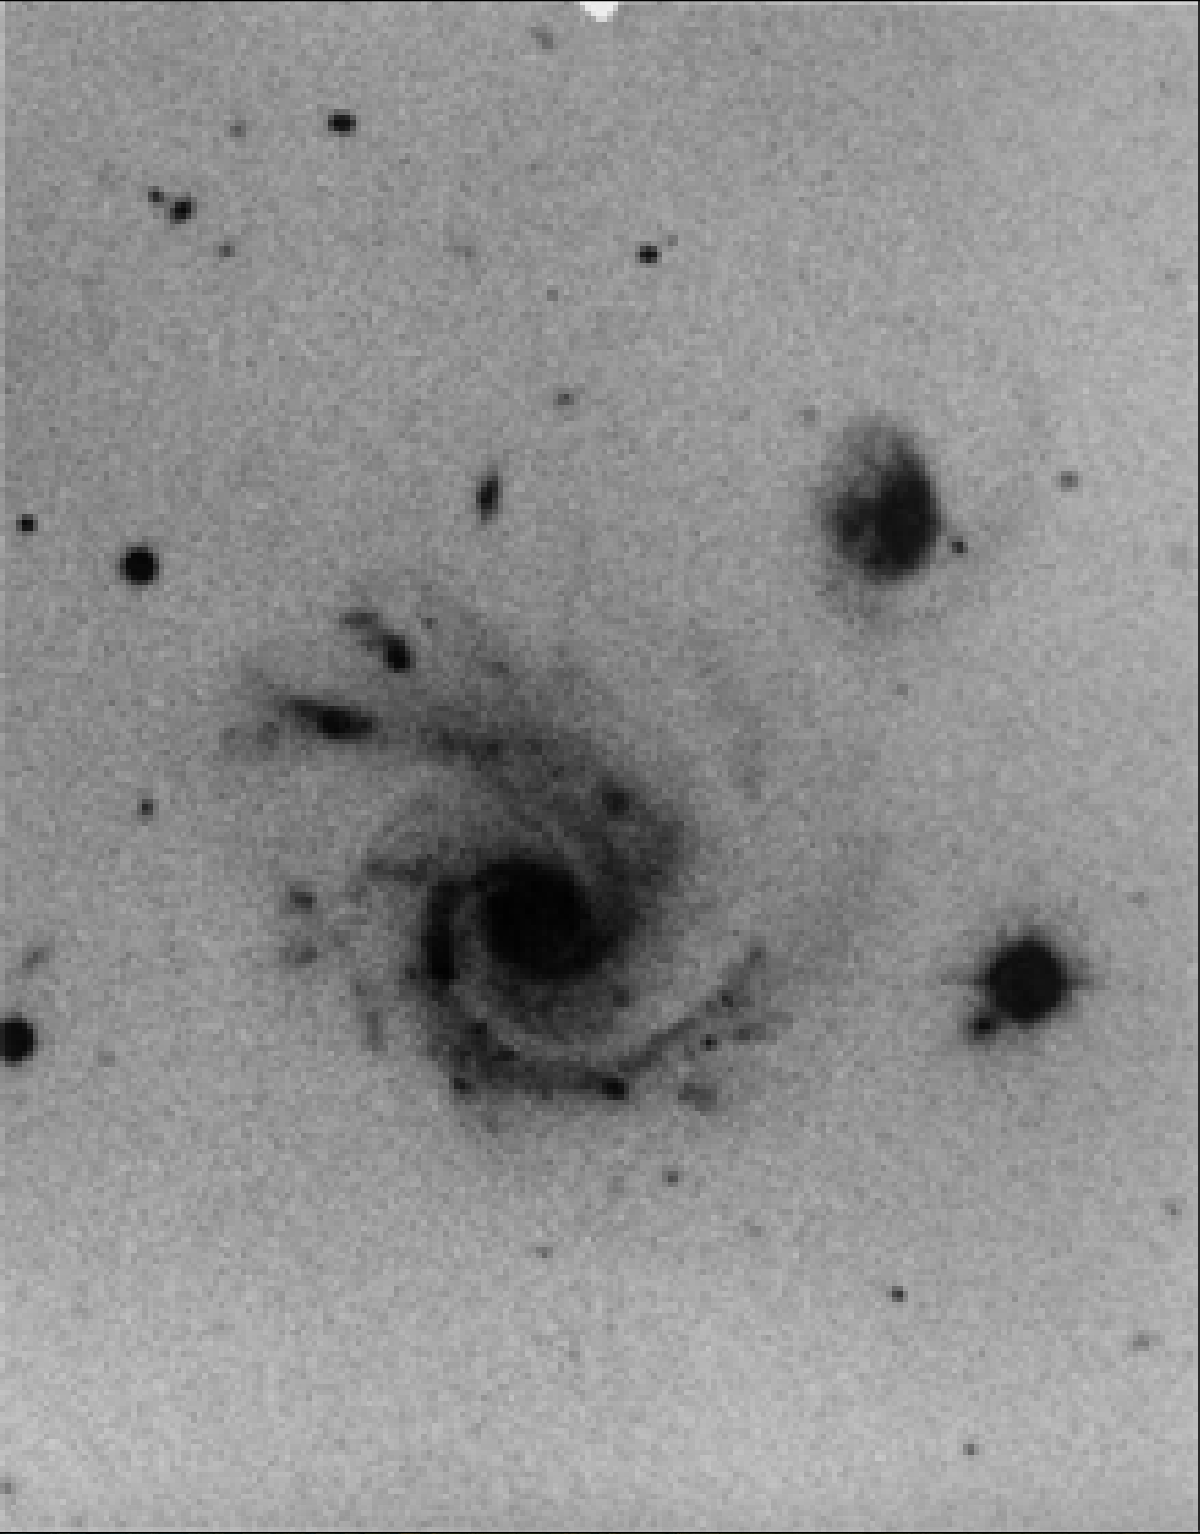
\includegraphics[scale=.50]{comparison_galaxy/arp_42.png}
    \caption{From Atlas Of Peculiar Galaxies, ARP 42}
    \label{fig:code}
\end{figure}





% E4
\begin{figure}[H]
    \centering
    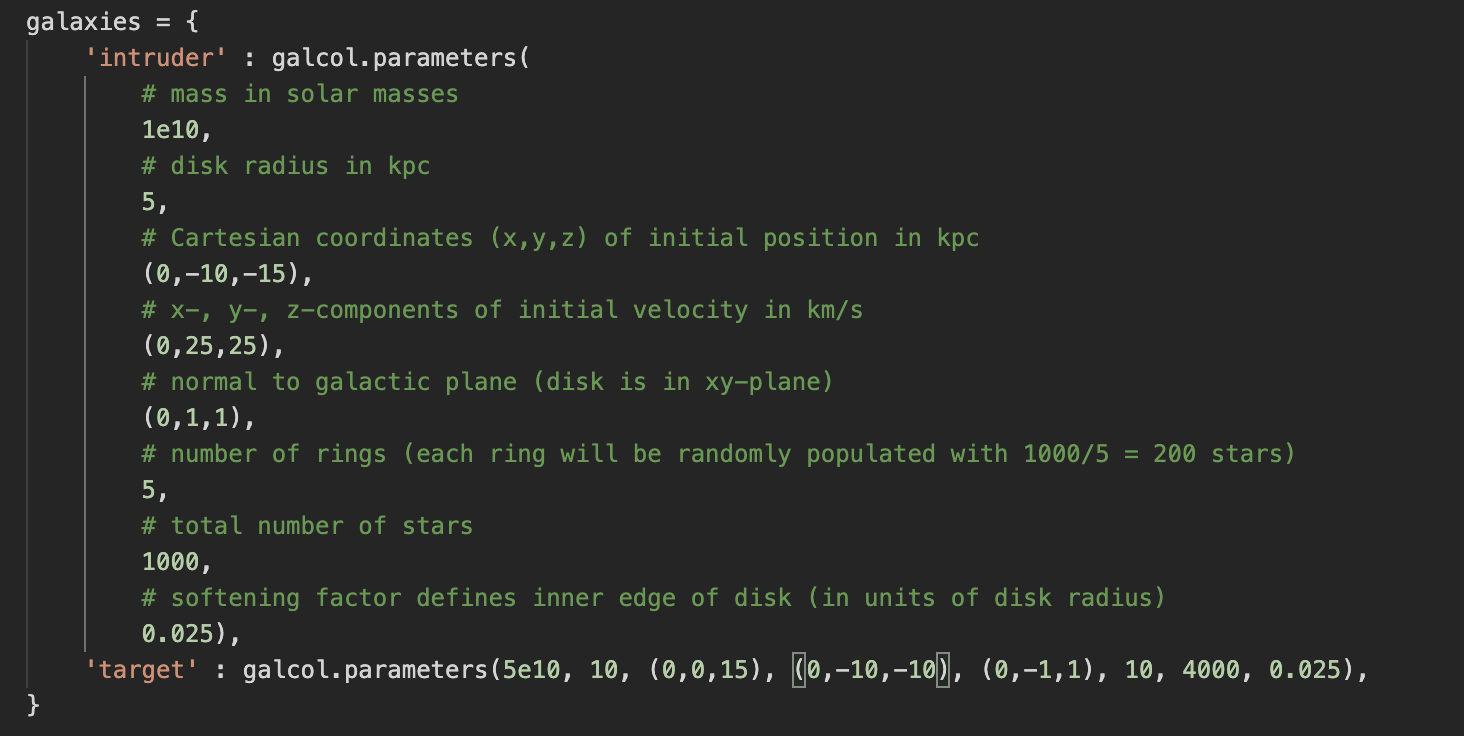
\includegraphics[scale=.60]{comparison_galaxy/ARP_50_vars.png}
    \caption{Varying position, velocity, and normal}
    \label{fig:code}
\end{figure}
\newpage
\begin{figure}[H]
    \centering
    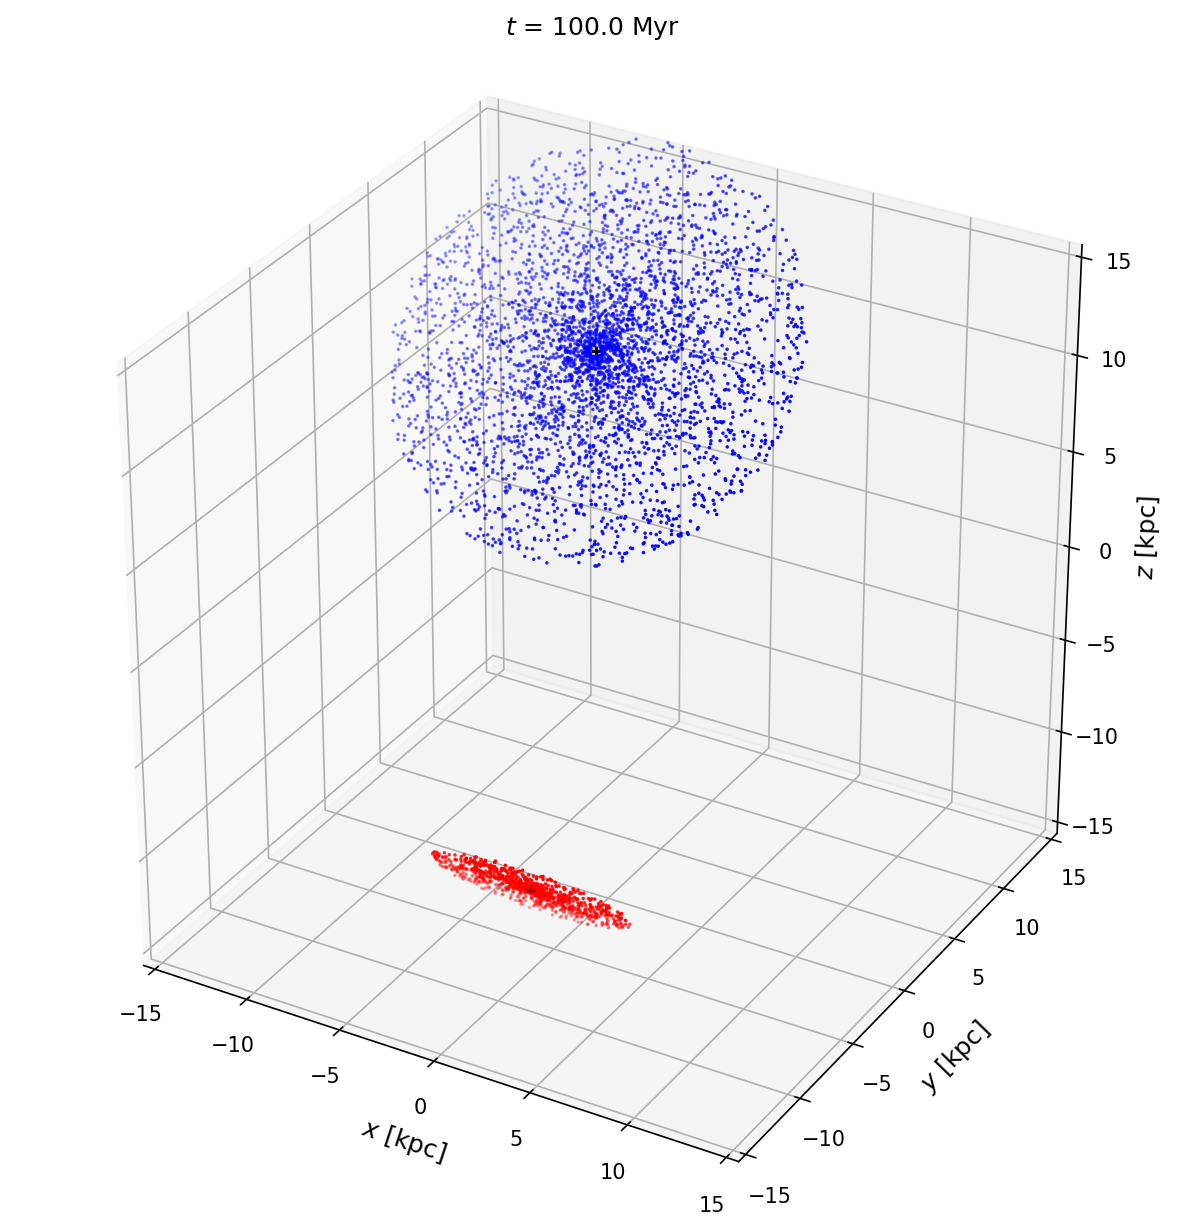
\includegraphics[scale=.40]{comparison_galaxy/ARP_50_input.png}
    \caption{Start}
    \label{fig:code}
\end{figure}
\begin{figure}[H]
    \centering
    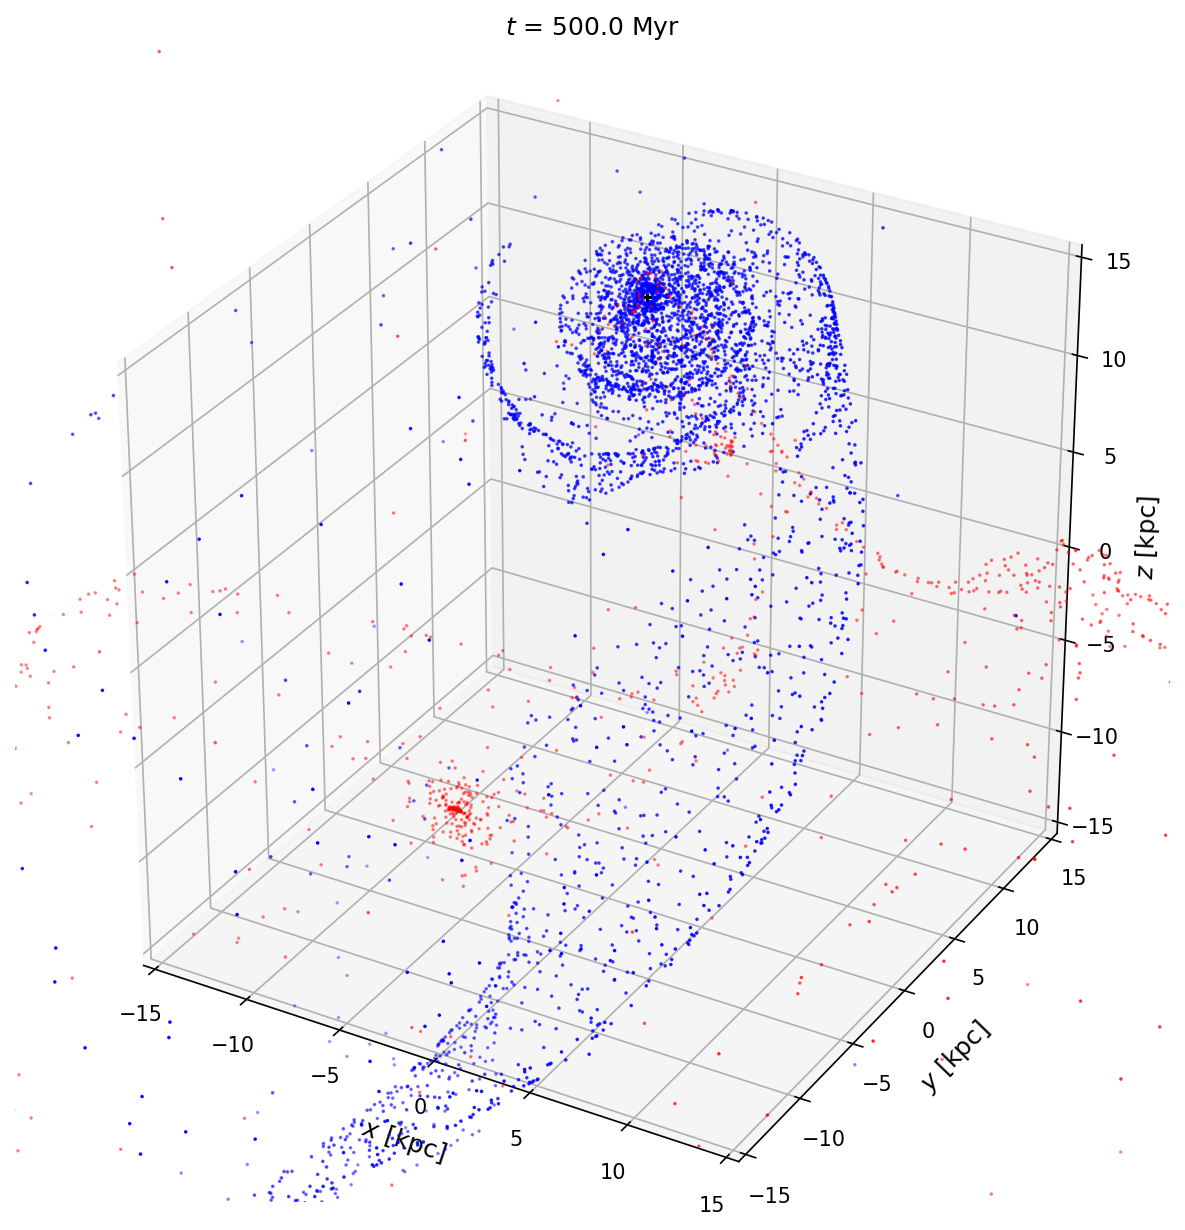
\includegraphics[scale=.40]{comparison_galaxy/ARP_50_output.png}
    \caption{Finish}
    \label{fig:code}
\end{figure}
\begin{figure}[H]
    \centering
    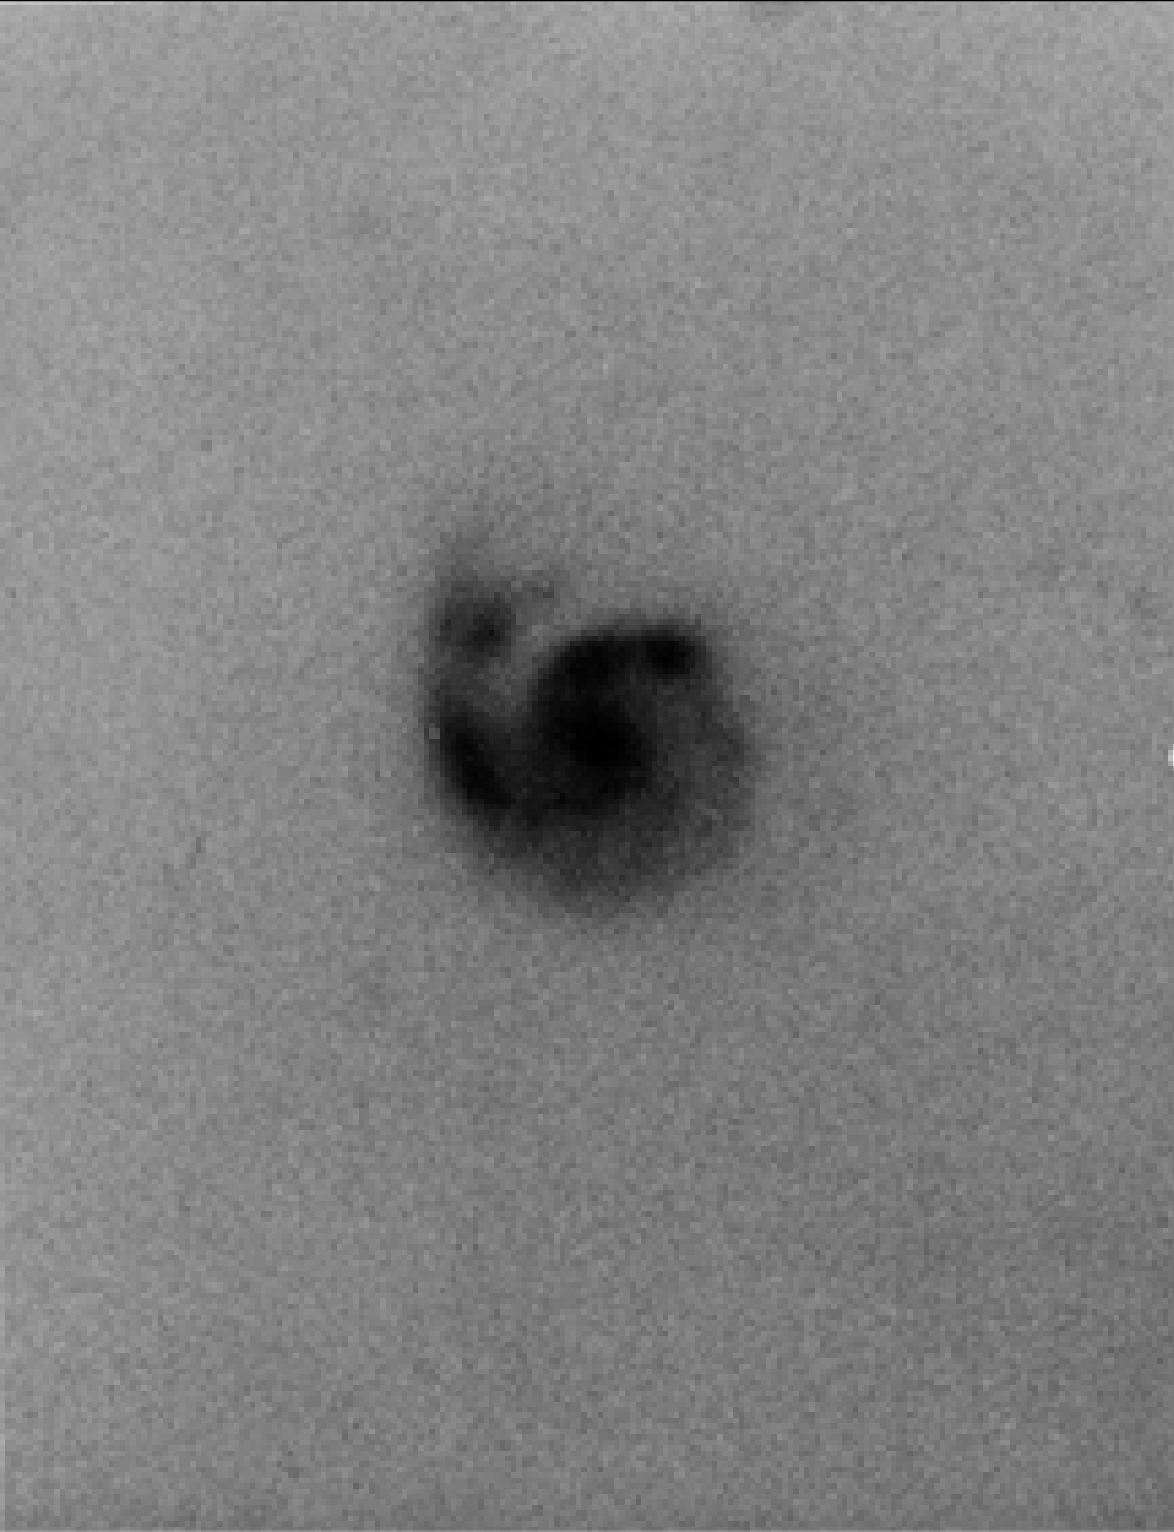
\includegraphics[scale=.50]{comparison_galaxy/arp_50.png}
    \caption{From Atlas Of Peculiar Galaxies, ARP 50}
    \label{fig:code}
\end{figure}





% E5
\begin{figure}[H]
    \centering
    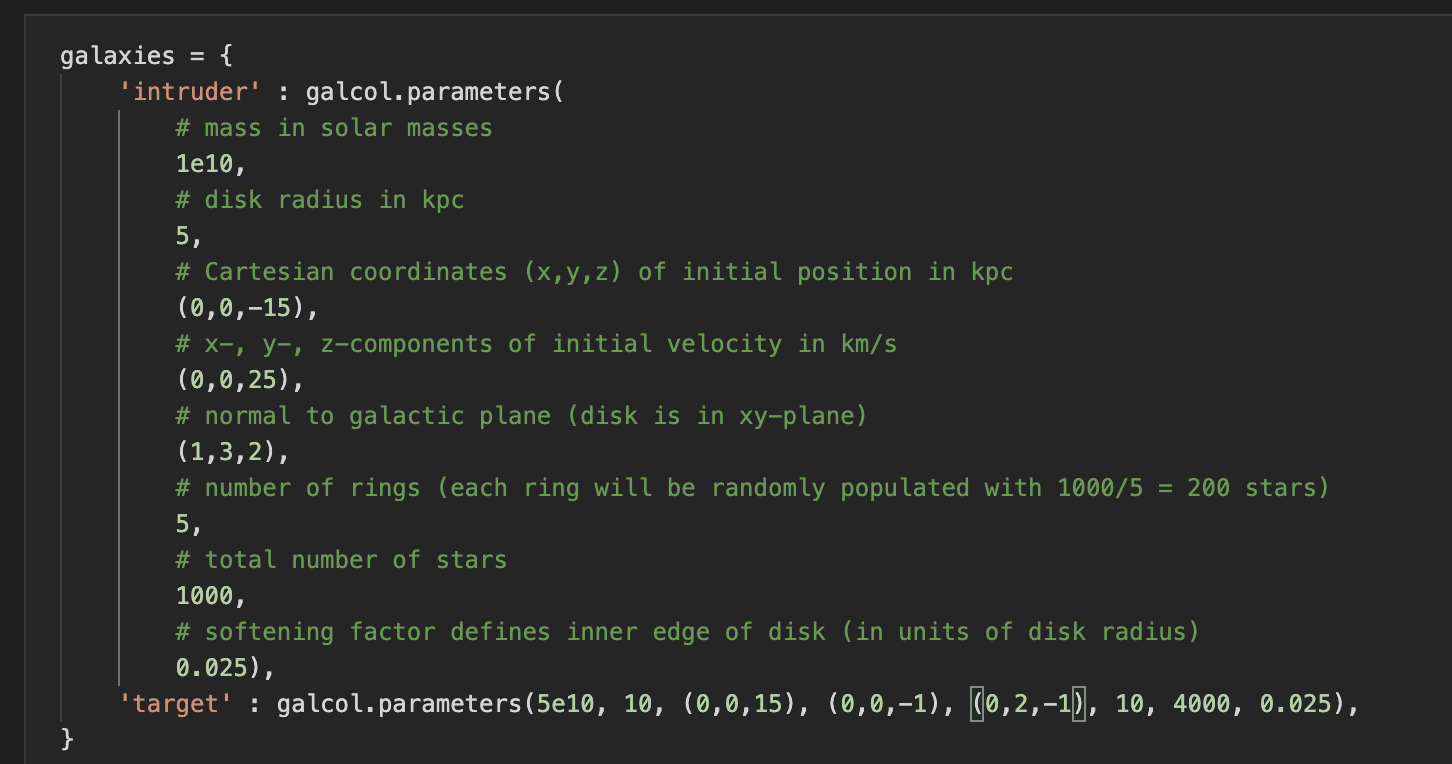
\includegraphics[scale=.60]{comparison_galaxy/ARP_66_vars.png}
    \caption{Varying position, velocity, and normal}
    \label{fig:code}
\end{figure}
\newpage
\begin{figure}[H]
    \centering
    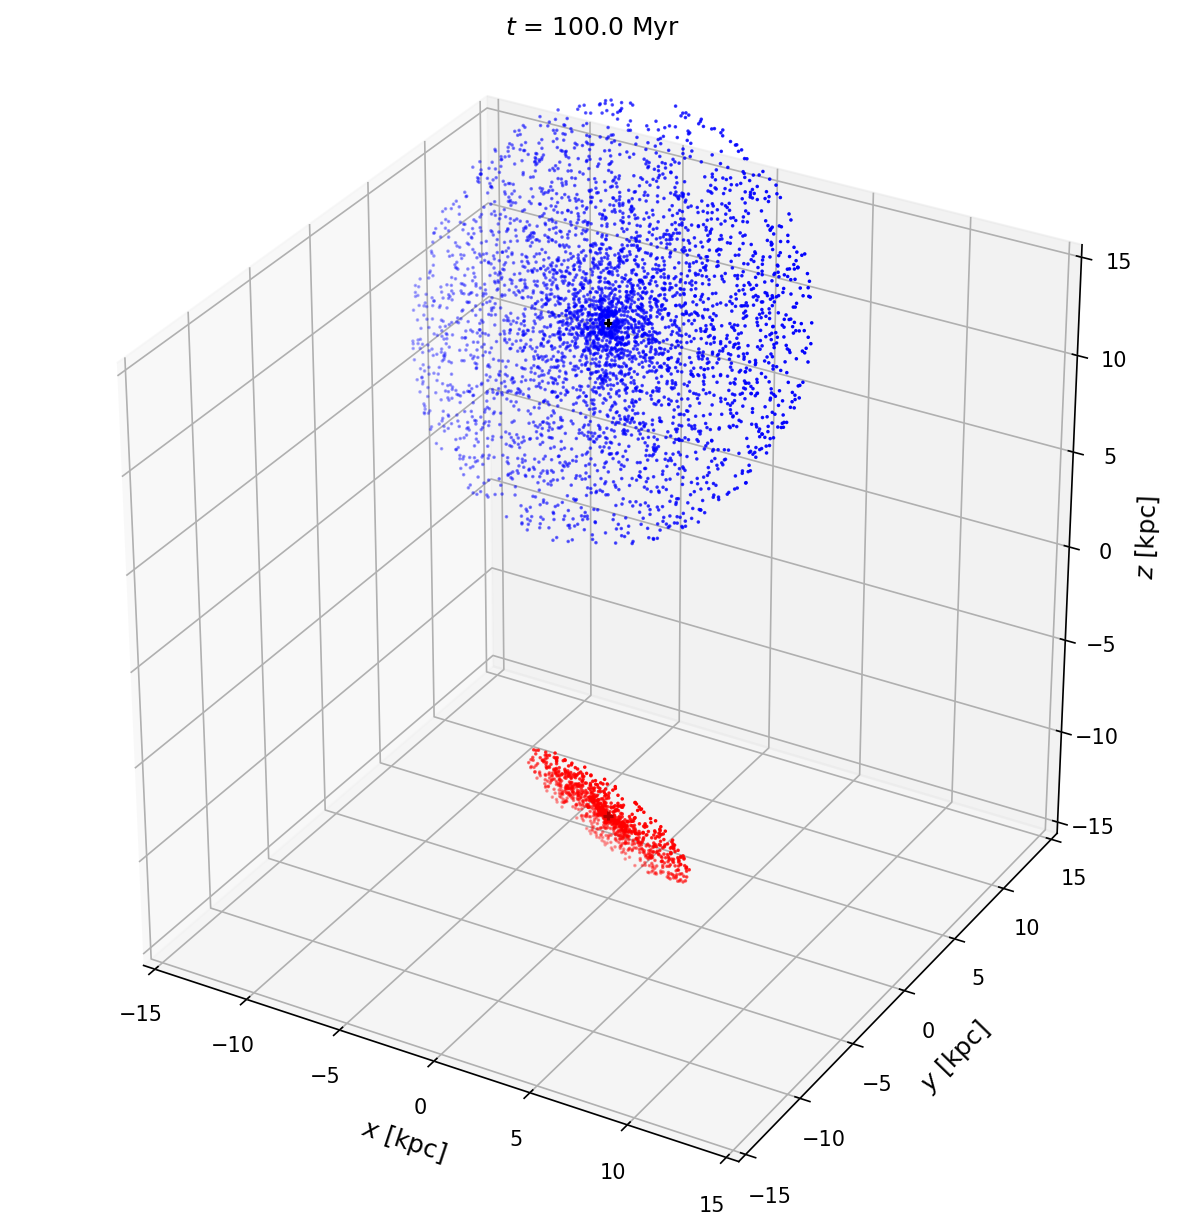
\includegraphics[scale=.40]{comparison_galaxy/ARP_66_input.png}
    \caption{Start}
    \label{fig:code}
\end{figure}
\begin{figure}[H]
    \centering
    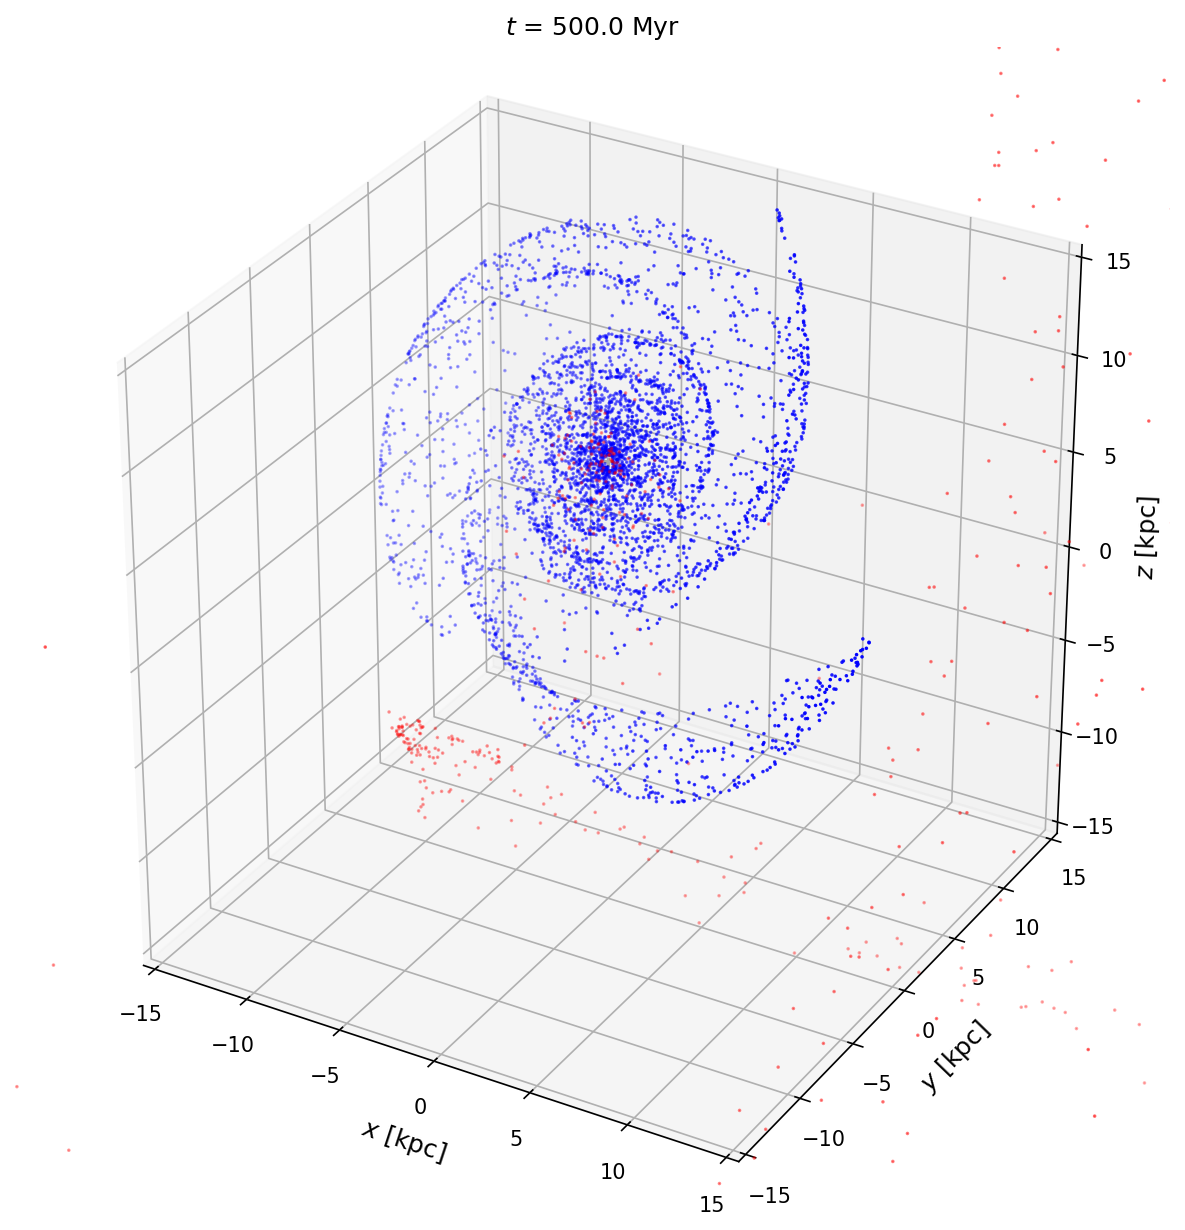
\includegraphics[scale=.40]{comparison_galaxy/ARP_66_output.png}
    \caption{Finish}
    \label{fig:code}
\end{figure}
\begin{figure}[H]
    \centering
    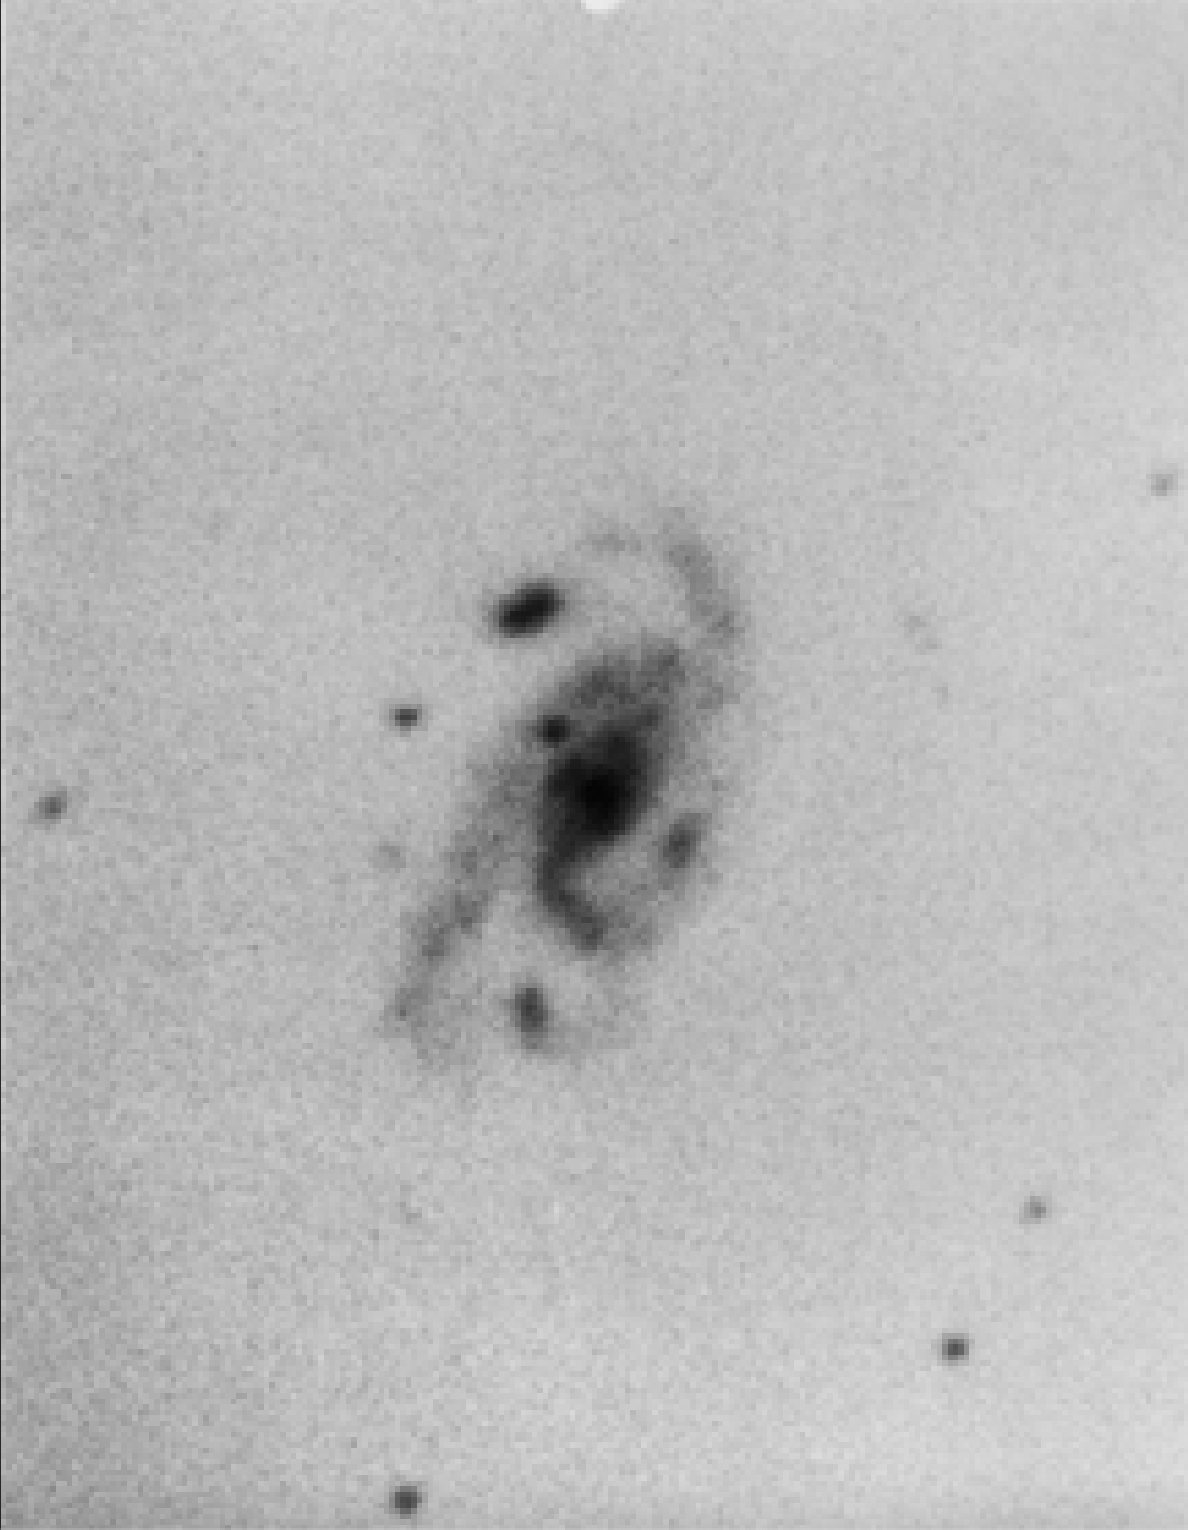
\includegraphics[scale=.50]{comparison_galaxy/arp_66.png}
    \caption{From Atlas Of Peculiar Galaxies, ARP 66}
    \label{fig:code}
\end{figure}





% E6
\begin{figure}[H]
    \centering
    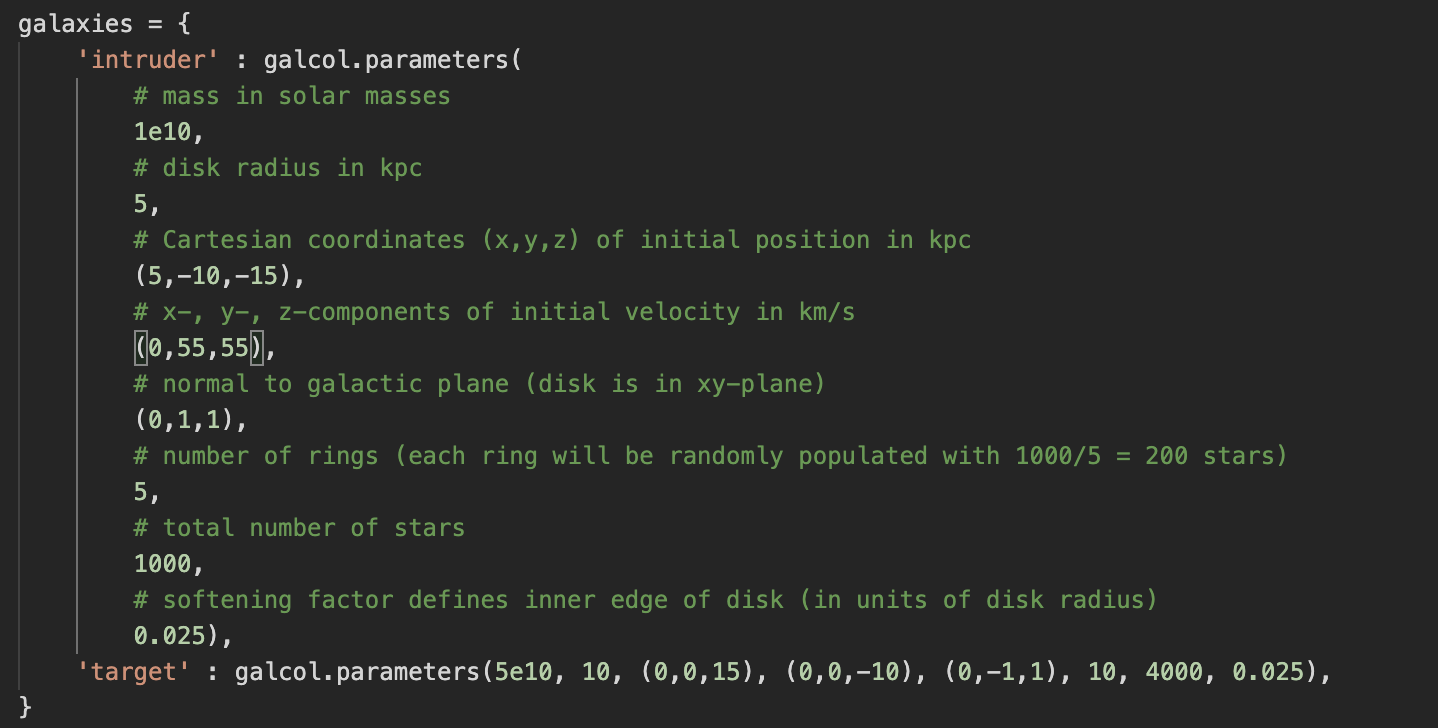
\includegraphics[scale=.60]{comparison_galaxy/ARP_70_vars.png}
    \caption{Varying position, velocity, and normal}
    \label{fig:code}
\end{figure}
\newpage
\begin{figure}[H]
    \centering
    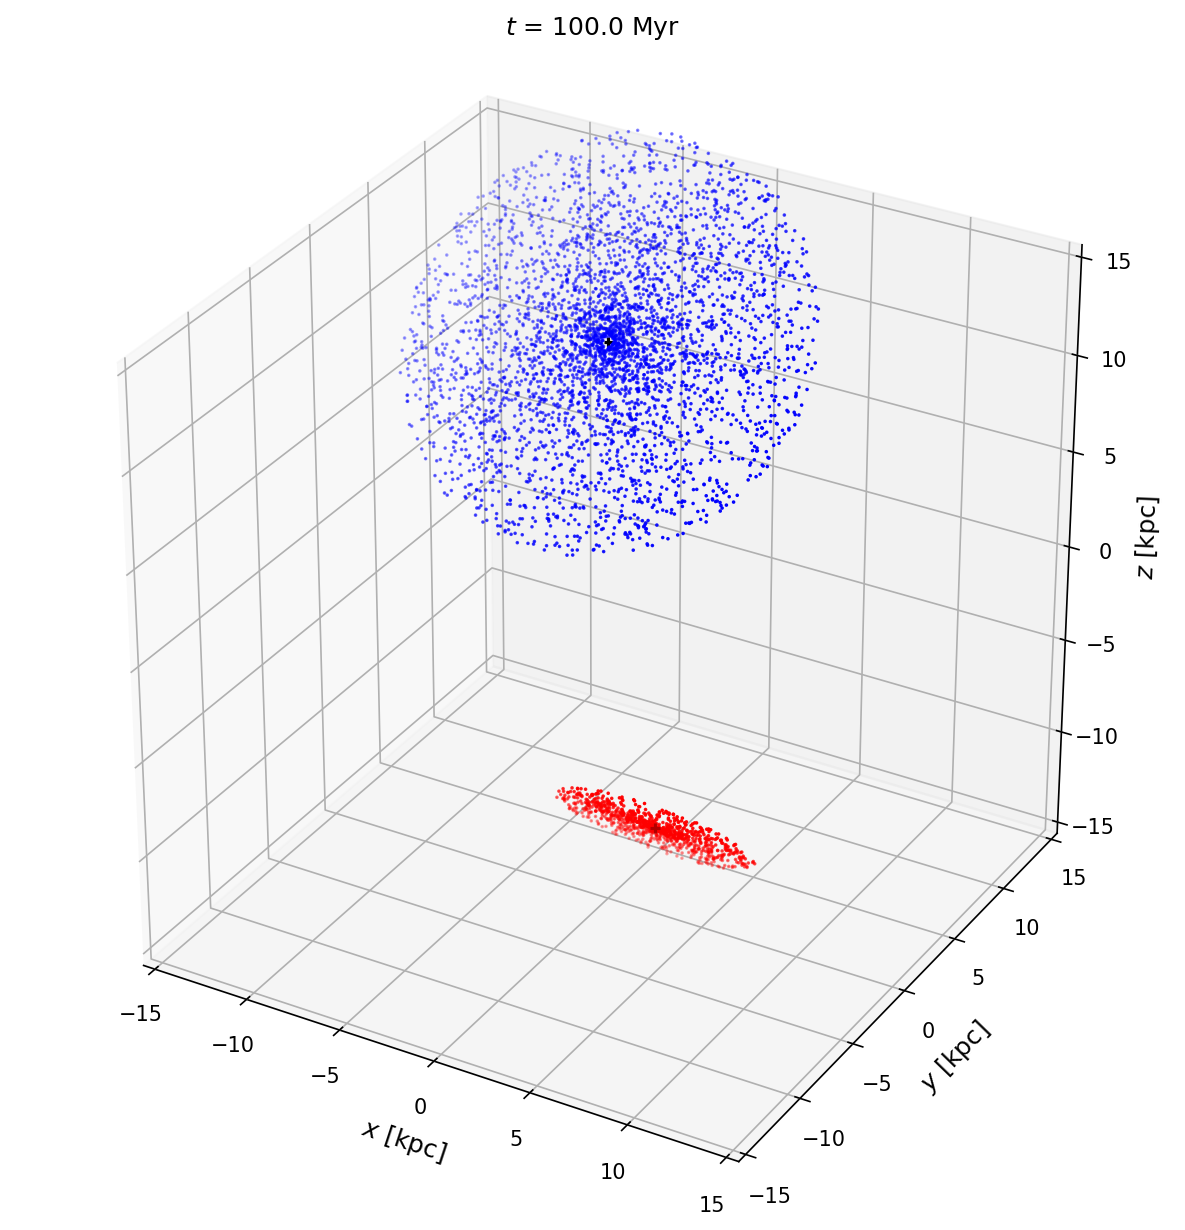
\includegraphics[scale=.40]{comparison_galaxy/ARP_70_input.png}
    \caption{Start}
    \label{fig:code}
\end{figure}
\begin{figure}[H]
    \centering
    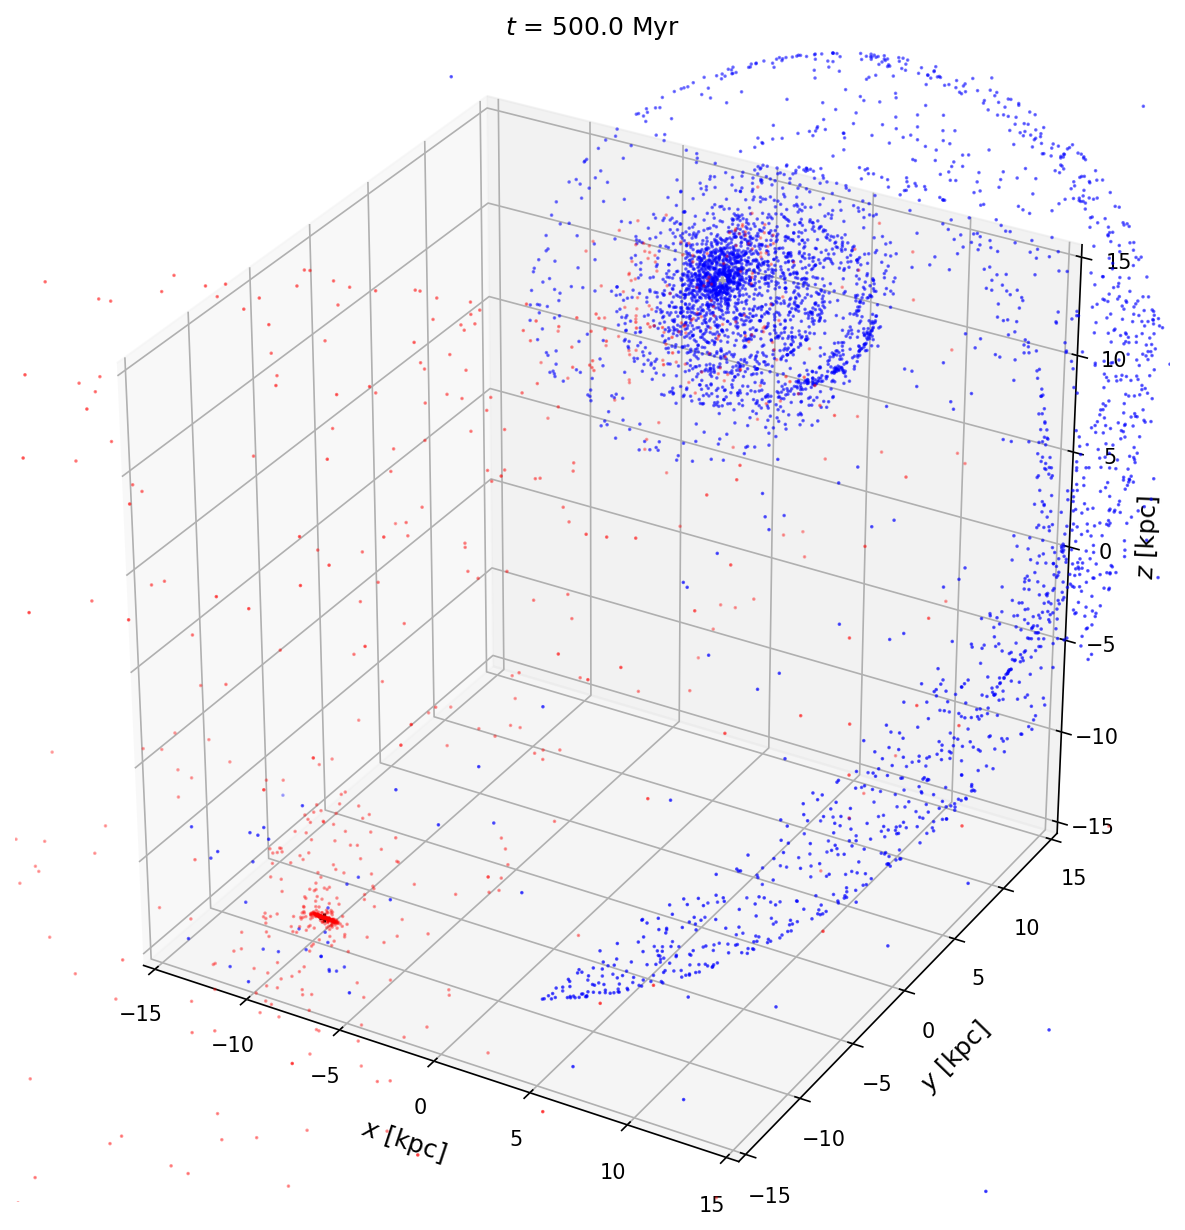
\includegraphics[scale=.40]{comparison_galaxy/ARP_70_output.png}
    \caption{Finish}
    \label{fig:code}
\end{figure}
\begin{figure}[H]
    \centering
    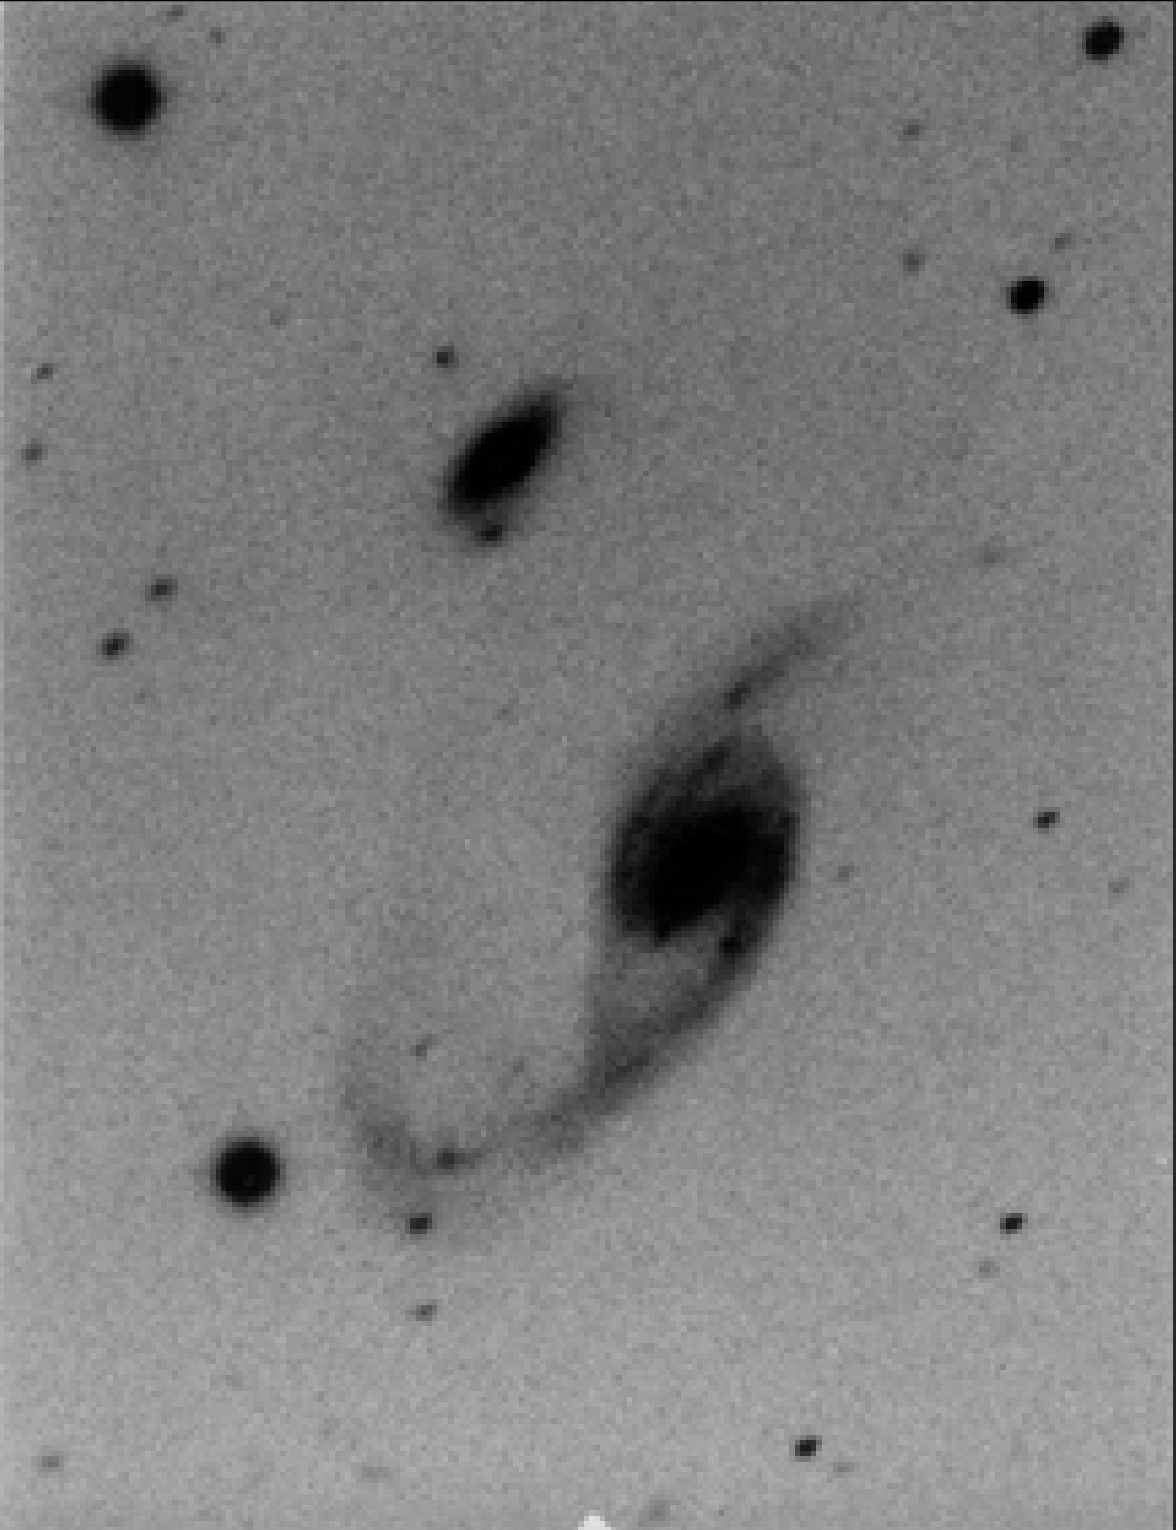
\includegraphics[scale=.50]{comparison_galaxy/arp_70.png}
    \caption{From Atlas Of Peculiar Galaxies, ARP 70}
    \label{fig:code}
\end{figure}

\section{Conclusion} \label{sec:results}
The N-body simulations of the galaxies proved to closely follow observed phenomena obtained from the  Atlas of Peculiar Galaxies. We successfully modeled a Cartwheel Galaxy (see: Figures 15-17). Additional variations in the velocity and angle of the galaxies successfully modeled various observed galaxy interactions (see: Figures 18-41). This demonstrates that the N-body simulation can show well the main components of galactic interactions. 

Although the N-body simulations followed very closely to the observed galaxy interactions, it does not completely capture galaxy interactions. This model made the assumption that there was no interaction between stars, all the mass is at the centers, and that there is no dark matter or interstellar medium. The first two assumptions are reasonable, as the effect of star interactions is negligible. However, further investigations should include the effects of dark matter and interstellar medium, like gas, dust, white dwarfs, planets, and dead stars between the stars to see how this affects the interaction and formation of stars. Trying different methods of the N-body simulation, such as the Tree-Code method, symplectic method, or SCF method, and comparing them to the code in this paper may lend to models of the interactions. The code was also limited in the number of particles the computer can handle. With recent developments in super-computing, further investigation can use the supercomputer to handle a wealth of particles when constructing the galaxy, creating a more accurate picture for galaxy interactions.

\newpage
\bibliographystyle{ieeetr}
\bibliography{citation.bib}

\section{Acknowledgements} \label{sec:acknowledgements}
We would like to express our gratitude to Brett Barkley and Dr. Shyamal Mitra for their guidance and lectures. 

\end{document}

